% Template:     Template Tesis LaTeX
% Documento:    Archivo principal
% Versión:      1.1.7 (02/10/2019)
% Codificación: UTF-8
%
% Autor: Pablo Pizarro R. @ppizarror
%        Facultad de Ciencias Físicas y Matemáticas
%        Universidad de Chile
%        pablo.pizarro@ing.uchile.cl, ppizarror.com
%
% Sitio web:    [https://latex.ppizarror.com/tesis]
% Licencia MIT: [https://opensource.org/licenses/MIT]
% CREACIÓN DEL DOCUMENTO
\documentclass[letterpaper,12pt,oneside]{book} % Libro, tamaño carta
\usepackage[utf8]{inputenc} % Codificación UTF-8

\bibliographystyle{unsrtnat}
% INFORMACIÓN DEL DOCUMENTO
\def\titulotesis {Modelamiento y seguimiento de tópicos para detección de modus operandi en robo de vehículos}
\def\titulogrado {
	Tesis para optar al grado de magíster en gestión de operaciones
	\bigbreak\vspace{0.3cm}
	Memoria para optar al título de ingeniero civil industrial
}

\def\nombreuniversidad {Universidad de Chile}
\def\nombrefacultad {Facultad de Ciencias Físicas y Matemáticas}
\def\departamentouniversidad {Departamento de Ingeniería Industrial}
\def\imagendepartamento {img/dptos/uchile2.pdf}
\def\imagendepartamentoescala {0.7}
\def\localizacionuniversidad {Santiago, Chile}

% INTEGRANTES, PROFESORES Y FECHAS
\def\autortesis {DIEGO GARRIDO}
\def\fechatesis {\the\year}

\def\tablacomision {
\begin{tabular}{c}
	\vspace{1.5cm} \\
	\MakeUppercase{\textbf{\autortesis}} \\
	\vspace{1.0cm} \\
	PROFESOR GUÍA: \\
	RICHARD WEBER \\
	\vspace{0.5cm} \\
	MIEMBROS DE LA COMISIÓN: \\
	PROFESOR 2 \\
	PROFESOR 3 \\
	\vspace{0.5cm} \\
	Este trabajo ha sido parcialmente financiado por: \\
	NOMBRE INSTITUCIÓN \\
	\vspace{0.5cm} \\
	\MakeUppercase{\localizacionuniversidad} \\
	\MakeUppercase{\fechatesis}
\end{tabular}}{
}
\def\tablaresumen {
\begin{tabular}{l}
	RESUMEN DE LA MEMORIA PARA OPTAR \\
	AL TÍTULO DE MAGÍSTER EN CIENCIAS \\
	DE LA INGENIERÍA \\
	POR: \MakeUppercase{\textbf{\autortesis}} \\
	FECHA: \MakeUppercase{\fechatesis} \\
	PROF. GUÍA: RICHARD WEBER
\end{tabular}}{
}

% CONFIGURACIONES
\input{lib/config}

% IMPORTACIÓN DE LIBRERÍAS
\input{lib/env/imports}
\graphicspath{img/} 

% IMPORTACIÓN DE FUNCIONES Y ENTORNOS
\input{lib/cmd/all}

% IMPORTACIÓN DE ESTILOS
\input{lib/style/all}

% CONFIGURACIÓN INICIAL DEL DOCUMENTO
\input{lib/cfg/init}

% TODONOTES
\usepackage{todonotes}

% INICIO DE LAS PÁGINAS
\begin{document}

% PORTADA
\input{lib/page/portrait} % Se puede borrar

% CONFIGURACIÓN DE PÁGINA Y ENCABEZADOS
\input{lib/cfg/page}

% DEDICATORIA
\begin{dedicatoria}
	Una frase de dedicatoria, \\
	pueden ser dos líneas. \newp
	\textbf{Saludos}
\end{dedicatoria}

% AGRADECIMIENTOS
\begin{agradecimientos}
    \todosec[inline]{TODO}
\end{agradecimientos}

% TABLA DE CONTENIDOS - ÍNDICE
\input{lib/page/index}

% RESUMEN O ABSTRACT
\begin{resumen}
    En este trabajo se describe una metodología para el descubrimiento de tópicos en el tiempo. La metodología propuesta está basada en (i) discretización del corpus en épocas, (ii) descubrimiento de tópicos en cada época mediante Hierarchical Dirichlet Process (HDP), (iii) la construcción de un grafo de similitud entre tópicos de épocas adyacentes, el cual permite modelar cambios entre los tópicos como: nacimiento, muerte, evolución, división y fusión. En contraste a trabajos anteriores, la metodología propuesta utiliza Word Mover's Distance (WMD) como medida de similitud entre tópicos, medida que destaca por ser robusta a tópicos que no poseen un vocabulario común, debido a que trabaja con sus \textit{word embeddings}. Se reportan resultados experimentales tanto cuantitativos como cualitativos en el fenómeno de robo de vehículos en Chile, usando como corpus los relatos de víctimas de robo de vehículo entre los años 2011-2016 provistos por la Asociación de Aseguradores de Chile (AACH). El algoritmo propuesto logra capturar bien los tópicos latentes del corpus, descubriendo delitos tales como \quotes{portonazo}, apropiación indebida y robo con violencia.
\end{resumen}

% CONFIGURACIONES FINALES
\input{lib/cfg/final}
\hypersetup{
    citecolor=Blue
}

% CONFIGURACIÓN TODONOTES 
% \reversemarginpar
% \setlength{\marginparwidth}{2.0cm}
% ======================= INICIO DEL DOCUMENTO =======================
\listoftodos
\chapter{Motivación}

Grandes volumenes de datos digitales son alamacenados día a día, en forma de noticias, blogs, páginas web, artículos científicos, libros, imágenes, sonido, video, redes sociales, etc. Volviéndose cada vez más difícil encontrar y descubrir lo que estamos buscando. Necesitamos herramientas computacionales que ayuden a organizar, buscar y entender grandes colecciones de datos.\\

Si pudieramos buscar y explorar documentos en base a sus temas, podríamos enfocar nuestra búsqueda en temas específicos o más amplios, podríamos observar como estos temas cambian en el tiempo o como se relacionan unos a otros. En vez de buscar documentos únicamente a través de palabras claves, podríamos primero hallar temas que son de nuestro interés, y luego examinar los documentos relacionados a ese tema. Por ejemplo, podríamos descubrir nuevas tendencias de investigación, analizar la evolución de la contigencia social, estudiar la efectividad de campañas publicitarias en base a la opinión de los consumidores, organizar y recomendar contenido en un blog, etc.\\

El objetivo del trabajo de tesis es desarrollar una metodología que permita descubrir tópicos en el tiempo, siendo capaz de modelar cambios tales como: nacimiento, muerte, evolución, división y fusión. Adicionalmente, que sea robusta a cambios en el vocabulario en el tiempo, permitiendo comparar tópicos entre épocas adyacentes a pesar que no posean un vocabulario común.

\section{Metodología Propuesta}
Los modelos de tópicos probabilísticos nos ayudan a descubrir los temas latentes (\textit{clusters}) en una colección de documentos, como estos temas están conectados unos a otros y cómo cambian en el tiempo. Permiten resumir un gran colección de documentos a través de sus temas y organizarlos entorno a estos.\\

Los modelos probabilísticos tratan un tópico como una distribución de probabilidad discreta sobre el vocabulario del corpus, siendo un práctica habitual interpretar un tópico a partir de sus $N$ palabras más probables. Por ejemplo, para $N=5$ las palabras más probables de un tópico son: \quotes{llaves}, \quotes{domicilio}, \quotes{individuos}, \quotes{casa} y \quotes{porton}, por lo que una etiqueta valida para este tópico podría ser \quotes{portonazo}.\\ 

En este trabajo se propone una metodología para el descubrimiento de tópicos en el tiempo. Esta metodología consiste en la discretización del corpus en épocas, el descubrimiento de tópicos en cada época mediante Hierarchical Dirichlet Process (HDP), la construcción de un grafo de similitud entre tópicos de épocas adyacentes, el cual permite modelar cambios entre los tópicos como: nacimiento, muerte, evolución, división y fusión. En contraste a trabajos anteriores, la metodología propuesta utiliza Word Mover's Distance (WMD) como medida de similitud entre tópicos. Esta medida destaca por su robustez ante tópicos que no poseen un vocabulario común, debido a que trabaja sobre el espacio de los \textit{word embeddings}.\\

\section{Caso de estudio}

Se escoge el problema del robo de vehículos o accesorios de vehículos como caso de estudio, debido a que es un problema que afecta a toda la sociedad en Chile y en el mundo, problema que se ha vuelto más relevante el último tiempo debido al crecimiento en el robo de vehículo motorizado y accesorios (ver Figura \ref{fig:antecedente}).\\ 

\begin{figure}
    \includegraphics[width=1\textwidth]{ch1/robberies.eps} 
    \caption{Cantidad de robos de vehículos y robos de accesorios de vehículos anuales en Chile entre los años 2006-2016. Fuente: Informe anual Carabineros, 2006-2016, INE.} 
    \label{fig:antecedente}
\end{figure}

Este fenómeno trae consigo un montón de costos para la sociedad, como incremento en la percepción de la seguridad, aumentos en la prima de los seguros de los asegurados, aumento en los costos de las aseguradoras \footnote{Considerando que el costo promedio incurrido en un auto asegurado robado y no recuperado es de \$ 5.000.000 de pesos, la pérdida total considerando solo los vehículos no recuperados para el año 2015 es de unos \$15.720 millones de pesos.} y el incremento de otros tipos de delitos \footnote{El destino de los vehículos robados es variado, se usan los autos para perpetrar otros delitos y huir, venderlos por piezas en talleres clandestinos o blanquear sus documentos para pasarlos por la frontera y venderlos o cambiarlos por droga en el extranjero.}

El corpus utilizado correspode a una colección de 49.015 relatos de víctimas de robo de vehículo, entre los años 2011-2016, provistos por la Asociación de Aseguradores de Chile (AACH). Cabe destacar que se estima que un tercio del parque automotriz se encuentra asegurado, por lo que se trabaja con una muestra del parque automotriz.\\
%http://www.economiaynegocios.cl/noticias/noticias.asp?id=185224

En el contexto de robo de vehículos, los tópicos vendrían siendo los \quotes{modu operandi} que utilizan los delicuentes para robar un vehículo. Así, la metodología propuesta permitiría descubrir los \textit{modus operandi} ocultos en los relatos de las víctimas y caracterizarlos a partir de las palabras, como también ver su evolución a través del tiempo, siendo capaz de detectar cuando nacen y mueren, y como cambian en el tiempo.\\

\section{Revisión del estado del arte}

El problema planteado consiste en un problema de \textit{clustering}, puesto que no se cuenta con una etiqueta del tema al que corresponde cada documento, siendo el propósito del trabajo descubrirla. Dentro de los métodos de \textit{clustering} que involucran texto el modelamiento de tópicos es uno de los enfoques más prometedores.\\

El modelamiento de tópicos es una poderosa herramienta que nos permite analizar grandes colecciones de documentos. En procesamiento de texto, un documento es una colección de palabras y el conjunto de documentos lleva por nombre corpus. Estos modelos encuentran los temas (\textit{clusters}) ocultos presentes en el corpus, permitiendo resumir, organizar y explorar grandes colecciones de datos.\\

Algunas de las técnicas de modelamiento de tópicos están basadas en factorización matricial como LSI (Latent Semantic Indexing) \citep{dumais2004latent} o NMF (Non-negative Matrix Factorization)\citep{xu2003document}, pero en este trabajo está basado en modelos probabilísticos generativos, como LDA (Latent Dirichlet Allocation)\citep{blei2003latent} o HDP (Hierarchical Dirichlet Process)\citep{teh2005sharing}. Ambos enfoques tienen sus pros y contras, en este trabajo se prefiere el enfoque probabilístico ya que es capaz de expresar incertidumbre en la asignación de un tópico a un documento y en la asignación de palabras a los tópicos, además, este enfoque suele aprender tópicos más descriptivos \citep{stevens2012exploring}.\\

En el modelamiento de tópicos se pueden presentar los siguientes dinamismos:
\begin{enumerate}
    \item \textbf{Evolución de los tópicos}: la evolución de los tópicos se refleja en el cambio en la distribución sobre las palabras. Por ejemplo, el \quotes{portonazo} en un determinado momento se comete en grupos de 2-3 personas con arma blanca, luego evoluciona de arma blanca a arma de fuego y lo perpetran jóvenes menores de edad.
    \item \textbf{Dinámismo en la mezcla de tópicos}: esto permite capturar la popularidad de los tópicos en el tiempo.
    \item \textbf{Nacimiento, muerte, fusión y división de tópicos}: En el contexto de robos es natural que en el tiempo aparezcan nuevos \textit{modus operandi} como también que desaparezcan aquellos que ya no parecen tan atractivos.
\end{enumerate}

En el modelamiento de tópicos estático destaca LDA y HDP. La diferencia principal en estos dos modelos es que el primero necesita de antemano fijar el número de tópicos a descubrir y el segundo lo infiere a partir del corpus.\\

Dentro de los primeros modelos de tópicos dinámicos que fueron exitosos podemos encontrar a Dynamic Topic Modelling (DTM) junto Topic Over Time (TOC)\citep{wang2006topics}. Estos modelos mantienen el número de tópicos fijo en el tiempo, por lo que si aparece un nuevo tópico este quedará clasificado dentro de un tópico preexistente desde el comienzo, por lo que solo es capaz de capturar el punto 1 y 2.\\

En \citep{ahmed2012timeline} se propone Dynamic Hierarchical Dirichlet Process (DHDP), modelo que no mantiene el número de tópicos fijo en el tiempo, sino que lo infiere a partir del corpus. Sin embargo, este modelo no es capaz de capturar fusión y división de tópicos. Además, a diferencia de los otros modelos de tópicos mencionados, DHDP no es una tecnología madura, puesto que no cuenta con una implementación disponible, por lo que se desconoce su desempeño en otras fuentes de información.\\

En \citep{wilson2011tracking} y \citep{beykikhoshk2018discovering} se propone una metodología que permite capturar los dinámismos mencionados utilizando LDA y HDP respectivamente. Estas consisten en dividir el corpus en épocas, entrenar de forma independiente un modelo de tópico en cada época, para finalmente unir los resultados obtenidos. En este trabajo se utilizan técnicas de modelado dinámico de tópicos bajo este enfoque, usando como HDP para el descubirmiento de tópicos en cada época.

\section{Estructura de la tesis}
En el capítulo \ref{ch:theorethical_framework} se describen los fundamentos teóricos en los que se basa la metodología propuesta la cual es descrita en el capítulo \ref{ch:methodology}. Luego, en el capítulo \ref{ch:case_study} se presenta un análisis cuantitativo y cualitativo de la metodología propuesta al fenómeno de robo de vehículos. Finalmente, en el capítulo \ref{ch:conclusion} se presentan las conclusiones y futuras lineas de investigación.

\chapter{Marco teórico}
\label{ch:theorethical_framework}

En este capítulo se describen los conceptos fundamentales para comprender la metodología propuesta en el capitulo \ref{ch:methodology}. El capítulo es estructurado como sigue. En la sección \ref{sec:mixture_models} se introducen a nivel general los modelos de \textit{clustering} probabiĺísticos conocidos como \textit{mixture models}. En la sección \ref{sec:topic_models} se introduce los modelos de tópicos LDA y HDP. Finalmente, en la sección \ref{sec:topic_evolution} se describe una metodología que modela la evolución en el tiempo una vez los tópicos son descubiertos. 

\section{Mixture Models}
\label{sec:mixture_models}

Uno de los supuestos básicos en \textit{clustering} es asumir que cada observación $x_{i}$ pertenece a un solo \textit{cluster} $k$. Podemos expresar la asignación a un \textit{cluster} como una variable aleatoria $z_{i}$, donde $z_{i}=k$ significa que $x$ pertenece al \textit{cluster} $k$, esta variable no es observada en los datos y se considera una variable oculta. Podemos obtener la distribución que caracteriza a un solo \textit{cluster} $k$ condicionando en $z_{i}$

\begin{align}
    p(x_{i}|z_{i}=k, \phi) & = p(x_{i}|\phi_{k})\\
\end{align}

Además, podemos definir la probabilidad de que una nueva observación pertenezca al \textit{cluster} $k$ 

\begin{align}
    p(z_{i}=k|\pi) & = \pi_{k}
\end{align}

$\sum_{k}\pi_{k} = 1$, ya que $\pi_{k}$ son probabilidades de eventos mutuamente excluyentes. La distribución de $x_{i}$ es entonces de la forma

\begin{align}
    p(x_{i}) = \sum_{k}\pi_{k}p(x_{i}|\phi_{k})
\end{align}

Podemos escribir $p(x_{i}|\phi_{k})$ como $x_{i} \sim F(\phi_{z_{i}})$, donde $F$ es la distribución asociada a las observaciones. \\

Una representación equivalente para este modelo viende de considerar que el parámetro $\bar{\phi_{i}}$ usado para generar la observación $x_{i}$ proviene de una distribucion discreta $G$, la cual tiene la forma

\begin{align}
    G(\phi) & = \sum_{k} \pi_{k}\delta_{\phi_{k}}(\phi)
\end{align}

Así, $G$ es una mezcla de funciones delta, donde la probabilidad que $\bar{\phi_{i}}$ es igual a $\phi_{k}$ es $\pi_{k}$. Luego, un \textit{mixture model} podría representarse como sigue

\begin{align}
\phi_{z_{i}} & \sim G\\
x_{i} & \sim  F(\phi_{z_{i}})
\end{align}

Un \textbf{Bayesian mixture model} es un \textit{mixture model} con una medida aleatoria para las mezclas. En la sección \ref{sec:dirichlet}. y \ref{sec:dp} nos referimos a dos priors ampliamente usados para construir \textit{bayesian mixture model}: la distribución Dirichlet que nos permite construir un \textbf{finite mixture model}, donde el número de átomos o \textit{clusters} a descubrir es finito, denotado por $K$ y un prior no paramétrico denominado Dirichlet Process (DP), el cual permite construir un \textbf{infinite mixture model}, donde el número de \textit{clusters} no está acotado. 

\subsection{Distribución Dirichlet}
\label{sec:dirichlet}

La distribución Dirichlet \citep{minka2000estimating} es una generalización multivariada de la distribución beta, la cual tiene soporte sobre un \textbf{simplex}, definido por:
\begin{equation}
    S_{K} = \{x: 0\leq x_{k} \leq 1, \sum_{k=1}^{K}x_{k}=1\}
\end{equation}
Luego, su función de densidad de probabilidad (pdf):

\begin{equation}
    Dir(x|\alpha)=\frac{1}{B(\alpha)}\prod_{k=1}^{K}x_{k}^{\alpha_{k}-1}\mathbb{I}(x\in S_{K})
\end{equation}

donde $B(\alpha) = B(\alpha_{1}, \ldots, \alpha_{K})$ es la generalización de la función beta a $K$ variables:

\begin{align}
    B(\alpha) \triangleq \frac{\prod_{k=1}^{K}\Gamma(\alpha_{k})}{\Gamma(\alpha_{0})}
\end{align}

donde $\alpha_{0} \triangleq \sum_{k=1}^{K}\alpha_{k}$.\\

En la Figura \ref{img:dirichlet_distribution} se observa el efecto de los parámetros en la distribución Dirichlet para $K=3$. Cuando $\alpha_{k}=1$ se tiene una distribución uniforme en el dominio $S_{K}$. El parámetro $\alpha_{k}$ controla la \textit{sparsity}, mientras más se acerca a 0 los vectores generados tienen más átomos nulos y se concentra la masa en unas pocas coordenadas, mientras más grande $\alpha_{k}$ la masa más se concentra en el centro (1/3, 1/3, 1/3), por último, cuando $\alpha$ no es simétrico la masa se concentra proporcionalmente en las coordenadas con $\alpha_{k}$ mayor.\\

\begin{figure}
    \centering
    \includegraphics[width=\textwidth]{ch2/dirichlet_simplex.eps}
    \caption{Densidad de la distribución Dirichlet para $K=3$ define una distribución sobre el \textit{simplex}, el cual puede ser representado por una superficie trinagular.}
    \label{img:dirichlet_distribution}
\end{figure}

En general se asume simetría en los parámetros de la distribución Dirichlet de la forma $\alpha_{k}=\frac{\alpha}{K}$, de esta manera $\alpha$ funciona como parámetro de concentración. En la Figura \ref{img:dirichlet_samples} se oberva una realización de una distribución Dirichlet para $\alpha \in \{0.1, 1, 10\}$ y $K\in\{2, 10, 100\}$, donde podemos observar que a mayor $\alpha$ los compenentes del vector $x$ más similares se vuelven, esto es más notorio a mayor dimencionalidad debido a que hay más dimensiones donde distribuir la masa.\\

La distribución Dirichlet es comúnmente usada en estadística Bayesiana, ya que es un prior conjugado con la distribución categórica (multinoulli) y la distribución multinomial. Así, la distribución Dirichlet puede ser utilizado como prior en un \textit{finite mixture model} asumiendo que $\pi\sim \text{Dir}(\frac{\alpha}{K}1_{K})$ y $\phi_{k} \sim H$.

\begin{figure}
    \centering
    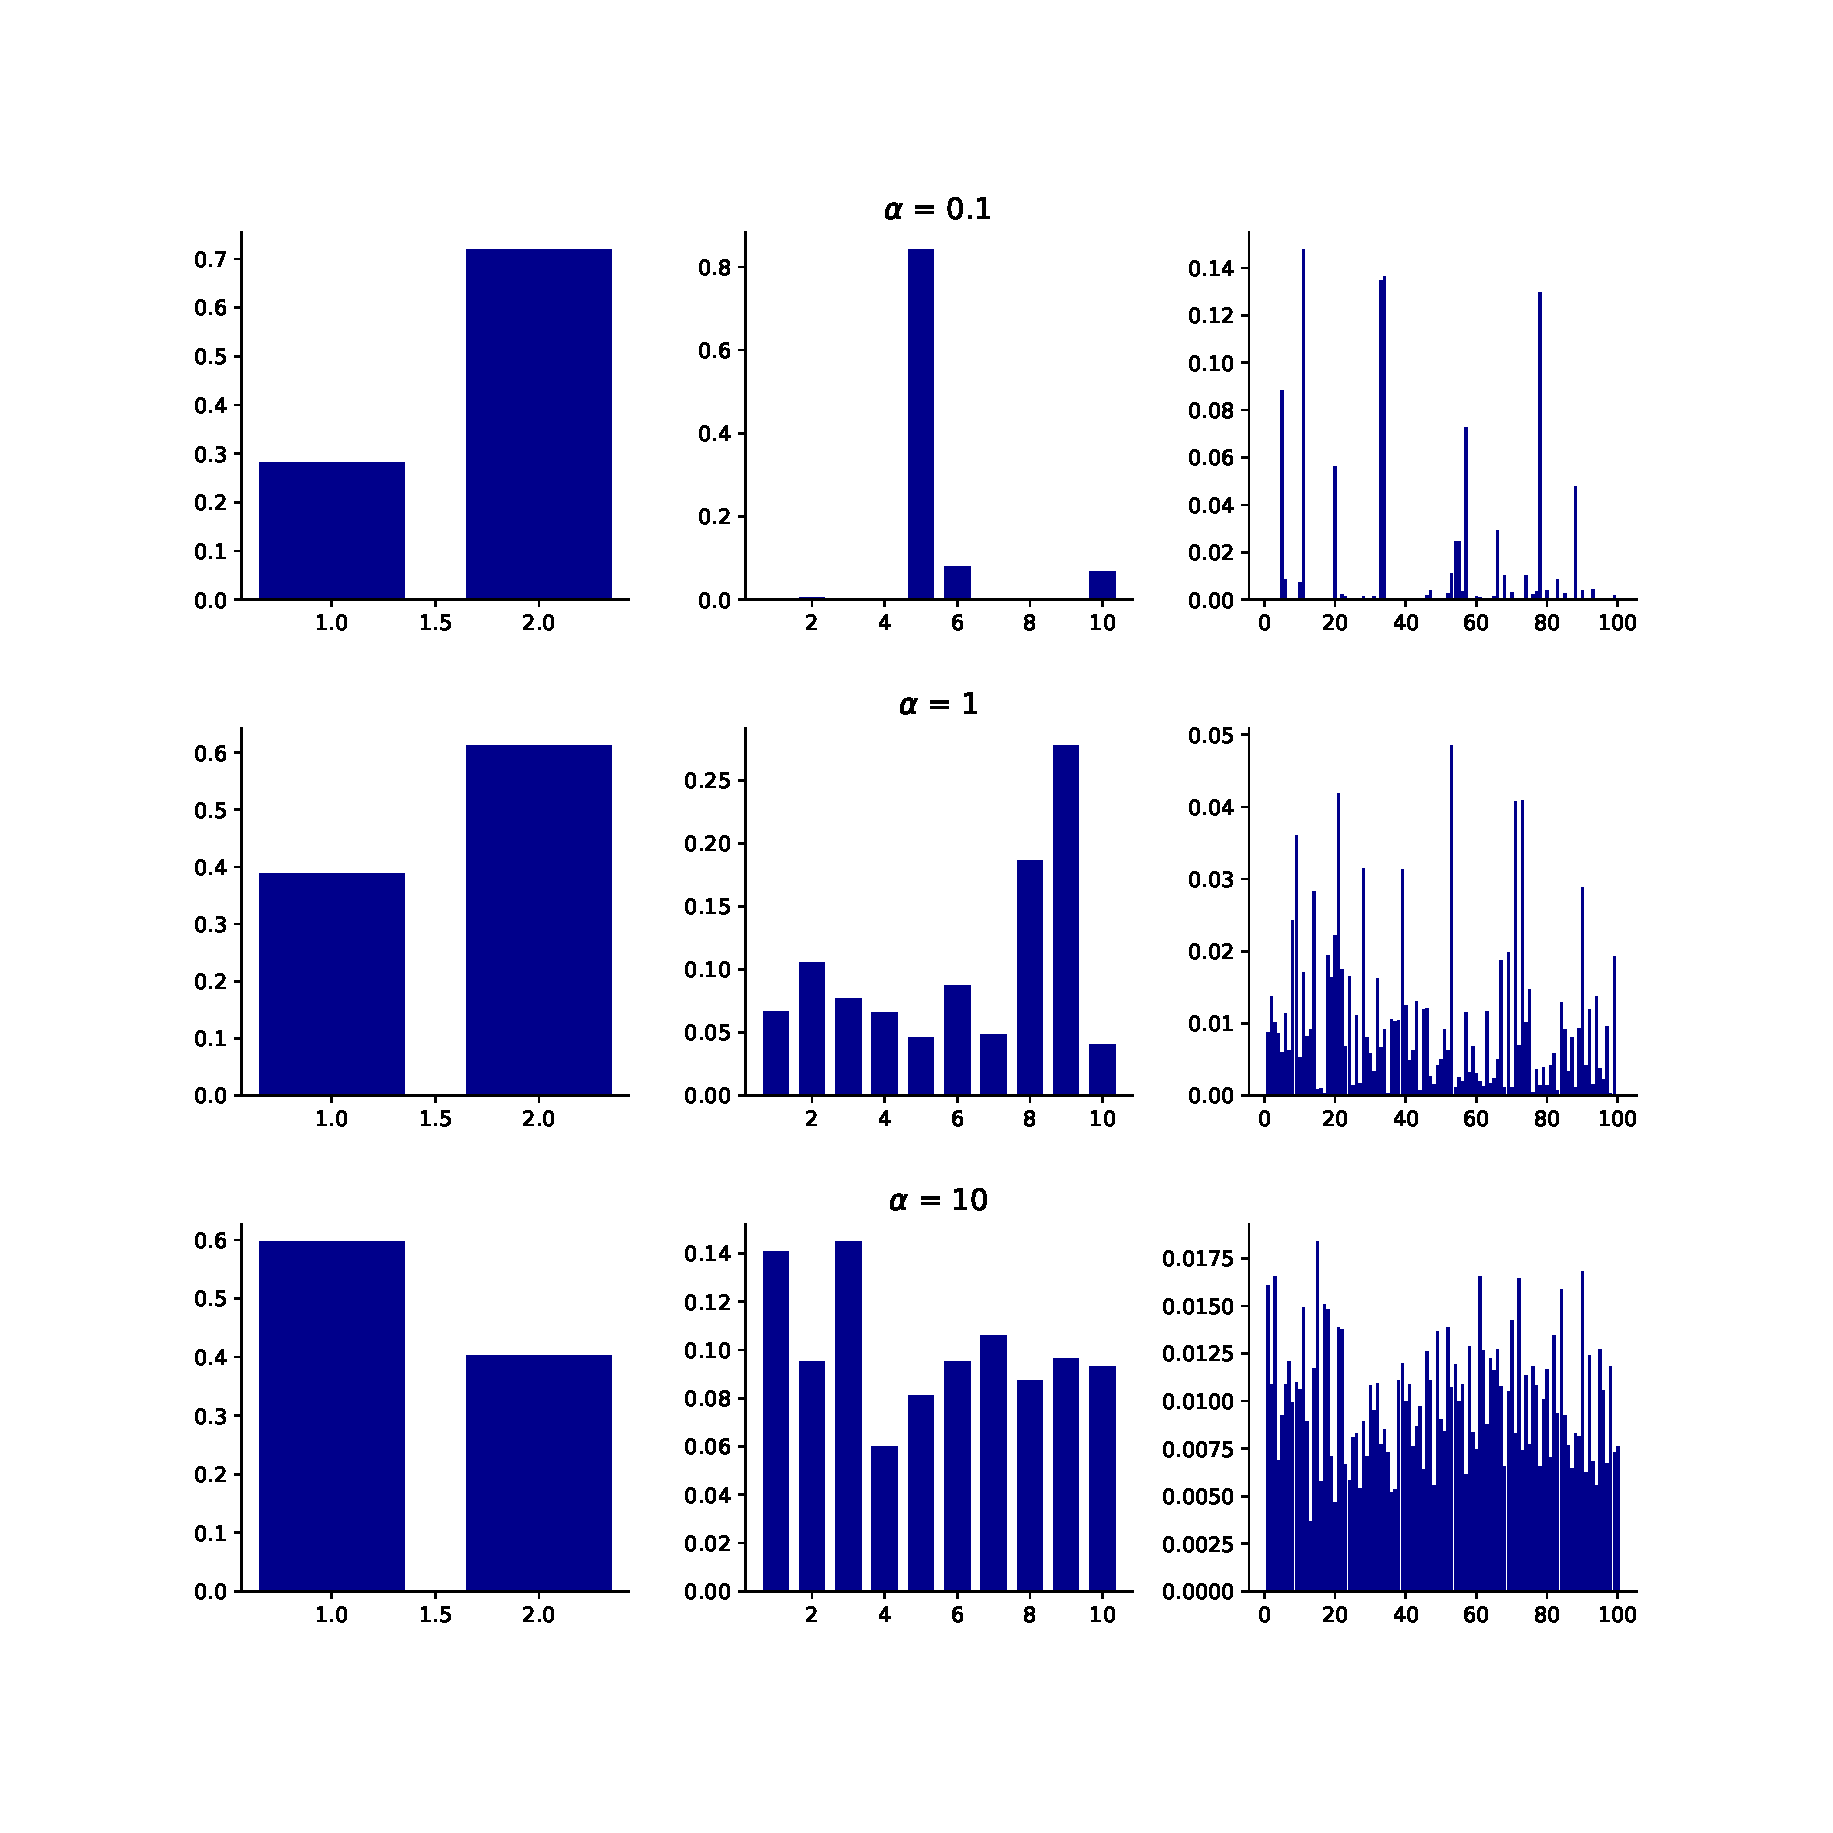
\includegraphics[width=\textwidth]{ch2/dirichlet_samples.eps}
    \caption{Muestra de una distribución Dirichlet simétrica para $\alpha \in \{0.1, 1, 10\}$ y $K\in\{2, 10, 100\}$.}
    \label{img:dirichlet_samples}
\end{figure}

\subsection{Dirichlet Process}
\label{sec:dp}

En un \textit{finite mixture model} tenemos $G(\phi) = \sum_{k=1}^{K} \pi_{k}\delta_{\phi_{k}}(\phi)$, luego si muestreamos a partir de $G$, con probabilidad uno obtendrémos exactamente $K$ \textit{clusters}. Nos gustaría tener un modelo más flexible, que pueda generar un número variable de \textit{clusters}. La forma de hacer esto es remplazar la distribución discreta $G$ por una medida aleatoria de probabilidad. El Dirichlet Process \citep{ferguson1973bayesian}, denotado $G\sim \text{DP}(\alpha, H)$, es una manera de hacer esto.\\

Un \textbf{Dirichlet Process} (DP) es una distribución sobre medidas de probabilidad $G: \Phi \rightarrow \mathbb{R}^{+}$, donde $G(\phi)\geq 0$ y $\int_{\Phi}G(\phi)d\phi=1$. Un DP se define implícitamente por cumplir 

\begin{align}
    G(A_{1}), \ldots, G(A_{K}) \sim \text{Dir}(\alpha H(A_{1}), \ldots, \alpha H(A_{K}))
\end{align}

para cualquier partición finita $(A_{1}, \ldots, A_{k})$ de $\Phi$. En este caso, decimos que $G\sim \text{DP}(\alpha, H)$, donde $\alpha$ es llamado el \textbf{parámetro de concentración} y $H: \Phi \rightarrow \mathbb{R}^{+}$ es llamado la \textbf{medida base}.\\

Como $p(G(A_{1}), \ldots, G(A_{K}))$ es Dirichlet, la distribución marginal en cada partición distribuye beta $\text{Beta}(\alpha H(A_{i}), \alpha \sum_{j\neq i}H(A_{j}))$. El DP es considerado consistentemente definido, en el sentido de que si particionamos $\bar{A}_{1}$ en $A_{1}$ y $A_{2}$, entonces $G(\bar{A}_{1})$ y $G(A_{1})+G(A_{2})$ siguen la misma distribución beta. \\

Sea $\phi \sim \text{Dir}(\alpha)$, y $z|\phi  \sim \text{Cat}(\pi)$, si integramos $\pi$ afuera obtenemos la distribución predictiva del modelo Dirichlet-multinoulli:
\begin{align}
    z\sim \text{Cat}(\alpha_{1}/\alpha_{0}, \ldots, \alpha_{K}/\alpha_{0})
\end{align}
donde $\alpha_{0} = \sum_{k}\alpha_{k}$. Es decir, $p(z=k|\alpha)=\alpha_{k}/\alpha_{0}$. Ademas, la posterior de $\pi$ dada una observación viene dada por
\begin{align}
    \pi|z \sim \text{Dir}(\alpha_{1}+\mathbb{I}(z=1), \ldots, \alpha_{K}+\mathbb{I}(z=K))
\end{align}

El DP generaliza el resultado anterior a particiones arbitrarias. Si $G\sim \text{DP}(\alpha, H)$, luego $p(\phi \in A_{i})=H(A_{i})$ y la posterior es

\begin{align}
    p(G(A_{1}), \ldots, G(A_{K})|\phi, \alpha, H) = \text{Dir}(\alpha H(A_{1})+\mathbb{I}(\phi \in A_{1}), \ldots, \alpha H(A_{K})+\mathbb{I}(\phi \in A_{K}))
\end{align}

Esto se mantiene para cualquier conjunto de particiones. Por lo tanto, si observamos multiples muestras $\bar{\phi}_{1:N}\sim G$, la nueva posterior está dada por 

\begin{align}
G|\bar{\phi}_{1:N}, \alpha, H \sim \text{DP}\bigg(\alpha+N, \frac{1}{\alpha+N}\bigg(\alpha H+\sum_{i=1}^{N}\delta_{\phi_{i}}\bigg)\bigg)
\end{align}

Por ende el DP define un prior conjugado para cualquier espacio medible, donde el parámetro de concentración $\alpha$ es como el tamaño de muestro efectivo de la medida base $H$.\\

Existen diferentes perspectivas que ayudan a entender la propiedad de \textit{clustering} de un Dirichlet Process. En la sección \ref{sec:sbp}. y \ref{sec:crp}. nos referimos a dos: el Stick Breaking Process y Chinese Restaurant Process (CRP).

\subsection{Stick Breaking Process}
\label{sec:sbp}

En esta sección describiremos una definición constructiva de un DP, conocida como \textit{stick breaking process} \citep{sethuraman1994constructive}. Sea $\pi=\{\pi_{k}\}_{k=1}^{\infty}$ una mezcla de pesos infinita derivada a partir del siguiente proceso:
\begin{align}
    \beta_{k} & \sim \text{Beta}(1, \alpha)\\
    \pi_{k} & = \beta_{k}\prod_{l=1}^{k-1}(1-\beta_{l}) = \beta_{k}(1-\sum_{l=1}^{k-1}\pi_{l})
\end{align}

Esto se suele denotar como $\pi \sim \text{GEM}(\alpha)$, donde GEM representa Griffiths, Engen y McCloskey, ver Figura  \ref{img:stick_breaking} para una ilustración. 

\begin{figure}
    \centering
    \includegraphics[width=0.6\textwidth]{ch2/stick_breaking.png}
    \caption{Ilustración de \textit{stick breaking process}. Tenemos una barra de largo 1, la cual se rompe en un punto aleatorio $\beta_{1}$, el largo de la pieza que conservamos es llamada $\pi_{1}$, luego recursivamente rompemos la barra restante, así generando $\pi_{2}, \pi_{3}, \ldots$. Fuente: Figura 2.22 de \citep{sudderth2006graphical}.}
    \label{img:stick_breaking}
\end{figure}

Algunos ejemplos de este proceso son mostrados en la Figura \ref{img:dp_samples} (a). A mayor $\alpha$, menos varianza y mayor número de átomos, por el contrario, pequeños valores de $\alpha$ muestran una alta varianza y menor número de átomos, adicionalmente exhiben mayor varianza en el número de átomos.

Se puede demostrar que este proceso terminará con probabilidad uno, a pesar que el número de elementos que este genera incrementa con $\alpha$. Además, el tamaño del componente $\pi_{k}$ decrece en promedio. Ahora definamos 
\begin{align}
    G(\phi) = \sum_{k=1}^{\infty}\pi_{k}\delta_{\phi_{k}}(\phi)
\end{align}

donde $\pi \sim \text{GEM}(\alpha)$ y $\phi_{k} \sim H$, se puede demostrar que $G \sim \text{DP}(\alpha, H)$. Como consecuencia de esta construcción, las muestras de un DP son \textbf{discretas con probabilidad uno}. En otras palabras, al ir muestreando $\bar{\phi_{i}}\sim G$ veremos valores repetidos, por lo que la mayoría de los datos vendrán de los $\phi_{k}$ con $\pi_{k}$ más largos. En la Figura \ref{img:dp_samples} (b) muestra un par de medidas aleatorias generadas a partir de un DP con una medida base normal.\\

\begin{figure}
    \centering
    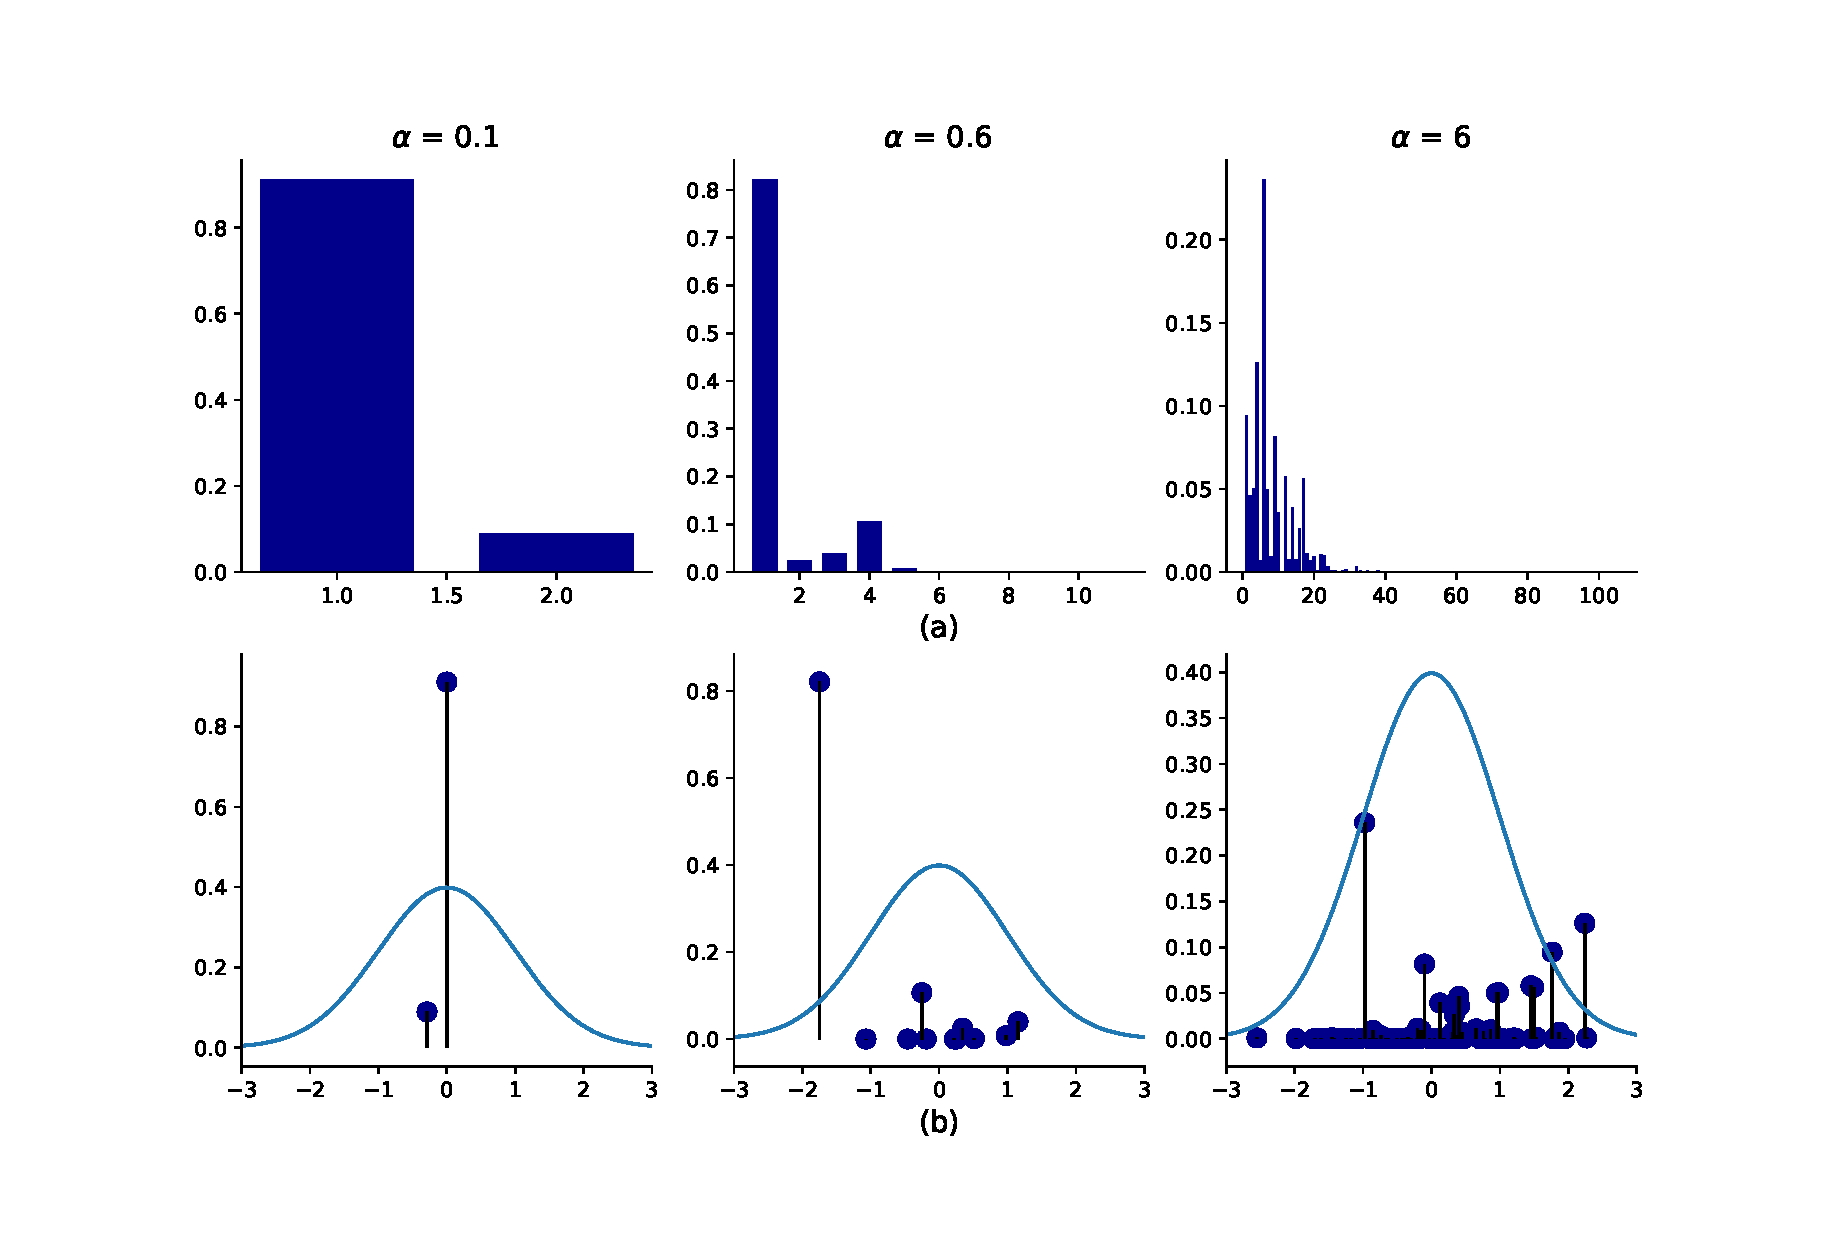
\includegraphics[width=\textwidth]{ch2/dp_samples.eps}
    \caption{(a) Muestra de una distribución GEM para diferentes parámetros de concentración $\alpha\in \{0.1, 0.6, 6\}$. (b) Medidas aleatorias generadas a partir de un Dirichlet Process con medida base normal $\mathcal{N}(0,1)$ para diferentes parámetros de concentración $\alpha\in \{0.1, 0.6, 6\}$}
    \label{img:dp_samples}
\end{figure}

\subsection{Chinese Restaurant Process}
\label{sec:crp}

Trabajar con infinitos átomos puede ser bastante problemático. Para sortear esta dificultad podemos explotar la propiedad de \textit{clustering} de un DP. Sea $\bar{\phi}_{1:N}\sim G$ observaciones generadas a partir de $G\sim \text{DP}(\alpha, H)$, sea $K$ los distintos valores de $\bar{\phi}_{1:N}$, luego la distribución predictiva condicionada en las $N$ observaciones está dada por

\begin{align}
p(\bar{\phi}_{N+1}=\phi|\bar{\phi}_{1:N}, \alpha, H) = \frac{1}{\alpha+N}\bigg(\alpha H(\phi)+\sum_{k=1}^{K}N_{k}\delta_{\bar{\phi}_{k}}(\phi)\bigg)
\end{align}

donde $N_{k}$ es el número de observaciones previas iguales a $\phi_{k}$. Esto esquema de muestreo es llamado \textit{Polya urn} o \textit{Blackwell-MacQueen}. Esta construcción provee una forma constructiva para muestrear de un DP. Es más conveniente trabajar con variables discretas $z_{i}$ que especifican cual valor de $\phi_{k}$ usar, así, definimos $\bar{\phi}_{i}=\phi_{z_{i}}$. Basado en esta expresión Tenemos

\begin{align}
p(z_{N+1}=z|z_{1:N}, \alpha) = \frac{1}{\alpha+N}\bigg(\alpha\mathbb{I}(z=k^{*})+\sum_{k=1}^{K}N_{k}\mathbb{I}(z=k)\bigg)
\end{align}

donde $k^{*}$ representa un nuevo \textit{cluster} que no ha sido usado aún. Este proceso es llamado Chinese Restaurant Process (CRP) \citep{aldous1985exchangeability}, basado en la oferta aparentemente infinito de mesas en ciertos restaurantes Chinos. La analogía es la siguiente: Las tablas del restaurante son los \textit{clusters}  y los clientes son las observaciones. Cuando una persona entra al restaurante, esta puede escoger sentarse en una tabla existente con probabilidad proporcional al número de personas ya sentadas en esa tabla ($N_{k}$), en otro caso, con una probabilidad decreciente a medida que más personas entran al restaurante (debido a $1/(\alpha +N))$ escogerá sentarse en una nueva tabla $k^{*}$. El resultado de este proceso es una distribución sobre particiones de los naturales, la cual es como una distribución de clientes a tablas.\\

El hecho de que las tablas actualmente ocupadas son más probables de obtener nuevos clientes se le suele llamar el fenómeno del \textit{rich get richer}. En efecto, se puede demostrar que la dsitribución del número de \textit{clusters} que induce este prior es básicamente una ley de potencia, donde el número de tablas $K$ con probabilidad 1 se aproxima a $\alpha log(N)$ cuando $N\rightarrow \infty$, mostrando que la complejidad del modelo crece logarítmicamente con el tamaño de los datos.

\section{Modelos de tópicos}
\label{sec:topic_models}
Los modelos de tópicos probabilísticos nos ayudan a descubrir los temas latentes (\textit{clusters}) en una colección de documentos, como estos temas están conectados unos a otros y cómo cambian en el tiempo. Permiten resumir un gran colección de documentos a través de sus temas y organizarlos entorno a estos.\\

Los modelos probabilísticos tratan un tópico como una distribución de probabilidad discreta sobre el vocabulario del corpus, siendo un práctica habitual interpretar un tópico a partir de sus $N$ palabras más probables. Por ejemplo, para $N=5$ las palabras más probables de un tópico son: \quotes{llaves}, \quotes{domicilio}, \quotes{individuos}, \quotes{casa} y \quotes{porton}, por lo que una etiqueta valida para este tópico podría ser \quotes{portonazo}.\\ 

En \textit{text mining} se suele trabajar bajo la asumpción de \textbf{bag of words} (bolsa de palabras), es decir, tanto los documentos como las palabras son tratadas como intercambiables. Es importante hacer notar que itercambiabilidad no es equivalente a que las variables aleatorias son independientes e identicamente distribuidas. Más bien, intercambiabilidad esencialmente puede ser interpretado como condicionalmente independientes e identicamente distribuidas, donde el condicionamiento es con respecto a los parámetros de una distribución de probabilidad. Por lo tanto, el supuesto de intercambiabilidad es claramente un supuesto de simplificación cuya principal justificación es la construcción de algoritmos computacionalmente más eficientes.\\

Un \textit{mixture model} bien conocido que trabaja bajo la asumpción de \textit{bag of words} es \textit{mixture of unigrams} \citep{nigam2000text}, el cual asume que todos los documentos provienen de un solo \textit{cluster} dentro de un conjunto finito de $K$ \textit{clusters}. Los documentos de un \textit{cluster} discuten solo un tópico particular $z$, y cada tópico $z$ está asociado a una distribución categórica. Así, la verosimilitud de observar un documento $d$ es

\begin{align}
    w|z &\sim \text{Cat}(\theta_{z})\\
    p(w_{1}, \ldots, w_{N_{d}}) &= \sum_{z=1}^{K}p(z)\prod_{i=1}^{N_{d}}p(w_{i}|z)
\end{align}

En comparación a \textit{mixture of unigrams}, LDA y HDP suponen que las palabras de un documento provienen de un mismo \textit{mixture model}. A nivel corpus los \textit{mixture models} comparten parámetros, que vienen siendo los tópicos, pero las \textit{mixtures of topics} son específicas de cada documento. Esto permite relajar la asumpción de que cada documento es generado por un solo tópico, permitiendo que un documento pueda tener presencia de más de un tema debido a que cada palabra proviene de algún tópico.\\

En las secciones \ref{sec:lda}-\ref{sec:hdp} se describe en detalle dos modelos de tópicos probabilísticos, Latent Dirichlet Allocation (LDA) y Hierarchical Dirichlet Process (HDP), considerado la generalización no parámetrica de LDA, donde el número de tópicos a descubrir no está acotado y se infiere a partir del corpus.\\

\subsection{Latent Dirichlet Allocation}
\label{sec:lda}

En Latent Dirichlet Allocation (LDA) \citep{blei2003latent} cada tópico es una distribución de probabilidad sobre un vocabulario fijo $V$. Cada documento $d$ tiene su propia mezcla de tópicos $\pi_{d}$. La asignación $z_{d,n}\in\{1, \ldots, K\}$  de de una palabra $n$ a un tópico $z$ es dibujada a partir de $\pi_{d}$. El modelo completo es como sigue

\begin{align}
    \phi_{k}|\eta \quad & \sim\quad \text{Dir}(\frac{\eta}{|V|}1_{|V|})\\
    \pi_{d}|\alpha \quad & \sim \quad \text{Dir}(\frac{\alpha}{K}1_{K})\\
    z_{d,n}|\pi_{d} \quad & \sim \quad \text{Cat}(\pi_{d})\\
    w_{d,n}|z_{d,n}, \phi_{1:K} \quad & \sim \quad \text{Cat}(\phi_{z_{d,n}})
\end{align}

Esto es ilustrado en la Figura \ref{img:lda}.
\begin{figure}
  \centering
  \tikz{ %

    \node[latent, dashed] (alpha) {$\alpha$} ; %
    \node[latent, right=of alpha] (pi) {$\pi_{d}$} ; %
    \node[latent, right=of pi] (z) {$z_{d,n}$} ; %
    \node[obs, right=of z] (w) {$w_{d,n}$}   ; %
    \node[latent, right=of w] (phi) {$\phi_{k}$} ; %
    \node[latent, right=of phi, dashed] (eta) {$\eta$} ;%
    \plate[inner sep=0.25cm, xshift=-0.12cm, yshift=0.12cm] {plate1} {(z) (w)} {$N_{d}$}; %
    \plate[inner sep=0.25cm, xshift=-0.12cm, yshift=0.12cm] {plate2} {(pi) (plate1)} {$D$}; %
    \plate[inner sep=0.25cm, xshift=-0.12cm, yshift=0.12cm] {plate3} {(phi)} {$K$}; %
    \edge {alpha} {pi} ; %
    \edge {pi} {z} ; %
    \edge {z,phi} {w} ; %
    \edge {eta} {phi} ; %
  }
\caption{Representación gráfica de LDA: círculos denotan variables aleatorias, círculos abiertos denotan parámetros, círculos sombreados denotan variables observadas y los platos indican replicación.}
\label{img:lda}
\end{figure}

La probabilidad conjunta del modelo:
\begin{equation}
    p(\phi, \pi, z, w|\alpha, \eta)= \prod_{k=1}^{K}p(\phi_{k}|\eta)\prod_{d=1}^{D}p(\pi_{d}|\alpha)\prod_{n=1}^{N_{d}}p(z_{n,d}|\pi_{d})p(w_{d,n}|\phi_{1:K}, z_{d,n})
\end{equation}

La distribución a posterior:
\begin{equation}
    p(\phi, \pi, z|w, \alpha, \eta) = \frac{p(\phi, \pi, z, w|\alpha, \eta)}{p(w|\alpha, \eta)}
\end{equation}

La distribución posterior es computacionalmente intratable para inferencia exacta, debido a que para normalizar la distribución debemos marginalizar sobre todas las variables ocultas y escribir la constante de normalización en términos de los parámetros del modelo. Para poder computar la posterior es necesario utilizar algoritmos de inferencia aproximada, donde el enfoque habitual es Markov Chain Monte Carlo (MCMC) \citep{andrieu2003introduction} e Inferencia Variacional (VI) \citep{blei2017variational}. En \citep{blei2003latent} se propone un algoritmo basado en VI y en \citep{griffiths2004finding} en MCMC.\\

Una representación equivalente en LDA sería generar cada palabra de un documento $d$ a partir de un tópico dibujado por una distribución $G_{d}$,

\begin{align}
    \phi_{k}|\eta \quad & \sim \quad \text{Dir}(\frac{\eta}{|V|}1_{|V|})\\
    \pi_{d}|\alpha \quad & \sim \quad \text{Dir}(\frac{\alpha}{K}1_{K})\\
    G_{d}(\phi)\quad & = \quad \sum_{k=1}^{K}\pi_{d, k}\delta_{\phi_{k}}(\phi)\\
    \phi_{d,n}|\pi_{d}, \phi_{1:K} \quad & \sim \quad G_{d}\\
    w_{d,n}|\phi_{d,n} \quad & \sim \quad  \text{Cat}(\phi_{d,n})
\end{align}

\subsection{Hierarchical Dirichlet Process}
\label{sec:hdp}

Hierarchical Dirichlet Process (HDP)\citep{teh2005sharing} es un prior no paramétrico, donde la medida base $G_{0}$ de un conjunto de DPs es dibujada a partir de un DP. En el caso de modelamiento de tópicos, temenos un medida global $G_{0}$ a nivel corpus que es dibujada a partir de un DP con medida base Dirichlet y una medida para cada documento que es dibujada a partir de un DP cuya medida base es $G_{0}$. El modelo completo es como sigue

\begin{align}
   H \quad &= \quad \text{Dir}(\frac{\eta}{|V|}1_{|V|})\\
   G_{0}|\gamma, H \quad &\sim \quad \text{DP}(\gamma, H)\\
   G_{d}|\alpha, G_{0} \quad &\sim \quad \text{DP}(\alpha_{0}, G_{0})\\
   \phi_{d,n}|G_{d} \quad &\sim \quad G_{d}\\
   w_{d,n}|\phi_{d,n} \quad &\sim \quad \text{Cat}(\phi_{d,n})
\end{align}

Esto es ilustrado en la Figura \ref{img:hdp}.

\begin{figure}
  \centering
  \tikz{ %
    \node[latent, dashed] (H) {$H$} ; %
    \node[latent, right=of H] (G0) {$G_{0}$} ; %
    \node[latent, above= of G0, dashed] (gamma) {$\gamma$} ; %
    \node[latent, right=of G0] (Gd) {$G_{d}$} ; %
    \node[latent, above= of Gd, dashed] (alpha0) {$\alpha_{0}$} ; %
    \node[latent, right= of Gd] (phi) {$\phi_{d,n}$} ; %
    \node[obs, right=of phi] (w) {$w_{d,n}$}   ; %
    \plate[inner sep=0.25cm, xshift=-0.12cm, yshift=0.12cm] {plate1} {(phi) (w)} {$N_{d}$}; %
    \plate[inner sep=0.25cm, xshift=-0.12cm, yshift=0.12cm] {plate2} {(Gd) (plate1)} {$D$}; %
    \edge {H, gamma} {G0} ; %
    \edge {G0, alpha0} {Gd} ; %
    \edge {Gd} {phi} ; %
    \edge {phi} {w} ; %
  }
\caption{Representación gráfica de HDP: círculos denotan variables aleatorias, círculos abiertos denotan parámetros, círculos sombreados denotan variables observadas y los platos indican replicación.}
\label{img:hdp}
\end{figure}

La discretitud a nivel corpus de $G_{0}$ asegura que todos los documentos comparten el mismo conjunto de tópicos (\textit{mixture components}). A nivel documento $G_{d}$ hereda los tópicos de $G_{0}$, pero los pesos de cada tópico (\textit{mixture proportions}) es específica del documento.\\


\subsubsection{Stick Breaking Construction}
Aplicando \textit{stick breaking construction} se tiene que para el DP dibujado a nivel corpus la siguiente representación:

\begin{align}
    \beta_{k}^{'} \quad &\sim \quad \text{Beta}(1, \gamma) \\
    \beta_{k} \quad &= \quad \beta_{k}^{'}\prod_{l=1}^{k-1}(1-\beta_{l}^{'})\\
    \phi_{k} \quad &\sim \quad H  \\
    G_{0}(\phi) \quad &= \quad \sum_{k=1}^{\infty}\beta_{k}\delta_{\phi_{k}}(\phi)
\end{align}

Así, $G_{0}$ es discreto y tiene soporte en los átomos $\phi = \{\phi\}_{k=1}^{\infty}$ con pesos $\beta=\{\beta_{k}\}_{k=1}^{\infty}$, siendo la distribución de $\beta$ escrita como $\beta \sim \text{GEM}(\gamma)$. La construcción a nivel documento de $G_{d}$ es:

\begin{align}
    \pi_{d,k}^{'} \quad &\sim \quad \text{Beta}\big(\alpha_{0}\beta_{k}, \alpha_{0}\big(1-\sum_{l=1}^{k}\beta_{l}\big)\big)\\
    \pi_{d,k} \quad &= \quad \pi_{d,k}^{'}\prod_{l=1}^{k-1}(1-\pi_{d,l}^{'})\\
    G_{d}(\phi) \quad &= \quad\sum_{k=1}^{\infty}\pi_{d,k}\delta_{\phi_{k}}(\phi)\\
    \phi_{d,n}|\pi_{d}, \phi_{1:\infty} \quad &\sim \quad G_{d}
\end{align}

Donde $\phi = \{\phi_{k}\}_{k=1}^{\infty}$ son los mismos átomos de $G_{0}$. Esto es ilustrado en la Figura \ref{img:hdp_sbc}.

%stick breaking
\begin{figure}
  \centering
  \tikz{ %
    \node[latent] (beta) {$\beta$} ; %
    \node[latent, above= of beta, dashed] (gamma) {$\gamma$} ; %
    \node[latent, right=of beta] (pi) {$\pi_{d}$} ; %
    \node[latent, above= of pi, dashed] (alpha0) {$\alpha_{0}$} ; %
    \node[latent, right= of pi] (z) {$z_{d,n}$} ; %
    \node[obs, right=of z] (w) {$w_{d,n}$}   ; %
    \node[latent, right=of w] (phi) {$\phi$} ; %
    \node[latent, above=of phi, dashed] (H) {$H$} ; %
    \plate[inner sep=0.25cm, xshift=-0.12cm, yshift=0.12cm] {plate1} {(z) (w)} {$N_{d}$}; %
    \plate[inner sep=0.25cm, xshift=-0.12cm, yshift=0.12cm] {plate2} {(pi) (plate1)} {$D$}; %
    \plate[inner sep=0.25cm, xshift=-0.12cm, yshift=0.12cm] {plate3} {(phi)} {$K (\infty)$}; %
    \edge {gamma} {beta} ; %
    \edge {beta, alpha0} {pi} ; %
    \edge {pi} {z} ; %
    \edge {z, phi} {w} ; %
    \edge {H} {phi} ; %
  }
\caption{Representación gráfica de la construcción stick-breaking de HDP: circulos denotan variables aleatorias, circulos abiertos denotan parámetros, círculos sombreados denotan variables observadas y los platos indican replicación.}
\label{img:hdp_sbc}
\end{figure}

\subsubsection{Chinese Restaurant Franchise Process}
%cite
Una construcción alternativa de HDP es conocida bajo el nombre de \textit{Chinese Restaurant Franchise Process} (CRF), una extensión del CRP, que permite compartir un conjunto de platos a través de una cadena de restaurantes Chinos. La analogía es la siguiente, tenemos $D$ restaurantes, cada uno con $N_{d}$ clientes $\phi_{d,i}$, que se sientan en tablas $t_{d,i}$, en cada tabla es servido un único plato $\phi_{k}\sim H$ a partir de un menú común para todos los restaurantes. \\

Sea $m_{dk}$ el número de tablas sirviendo el plato $k$ en el restaurante $d$, así $m_{d.}$ representa el número de tablas en el restaurante $d$, $m_{.k}$ representa el número de tablas sirviendo el plato $k$, y $m_{..}$ el número total de tablas ocupadas. Primero, procedemos a integrar afuera $G_{d}$, siendo la probabilidad condicional del cliente $i$ en la tabla $t$

\begin{align}
p(t_{di}=t|t_{d1}, \ldots, t_{d,i-1}, \alpha_{0}, G_{0}) = \frac{1}{\alpha_{0}+i-1}\bigg(\alpha_{0}\mathbb{I}(t=t^{*})+\sum_{t^{'}=1}^{m_{d.}}N_{dt^{'}}\mathbb{I}(t=t^{'})\bigg)
\end{align}

donde $N_{dt^{'}}$ representa los clientes del restaurante $d$ que están sentados en la tabla $t^{'}$. Con probabilidad proporcional a los clientes sentados en la tabla $t$ los clientes del restaurante se sentarán en esta y con probabilidad proporcional a $\alpha_{0}$ en una nueva. Una vez todos los clientes estan sentados tenemos una partición sobre $\phi_{d1}, \ldots, \phi_{dN_{d}}$ para cada documento $d$. Luego, procedemos a integrar afuera $G_{0}$, obteniéndose

\begin{align}
    p(z_{dt}=z|z_{11}, z_{12}, \ldots, z_{d1}, \ldots, z_{d, t-1}|\gamma, H) = \frac{1}{\gamma+m_{..}}\bigg(\gamma\mathbb{I}(z=k^{*})+\sum_{k=1}^{K}m_{.k}\mathbb{I}(z=k)\bigg)
\end{align}

en este caso se tiene que la tabla $t$ del restaurante $d$ con probabilidad proporcional al número de tablas que sirven el plato $k$ ($m_{.k}$) servirá el plato $k$ y con probabilidad proporcional a $\gamma$ servirá un nuevo plato.\\

Al igual que LDA la distribución posterior es intratable, en  \citep{teh2005sharing} se propone un algoritmo basado en MCMC bajo la construcción CRF de un HDP. 

\section{Modelamiento de la evolución de los tópicos en el tiempo}
\label{sec:topic_evolution} 

En \citep{wilson2011tracking} y \citep{beykikhoshk2018discovering} se propone una metodología que permite capturar los dinámismos mencionados usando LDA y HDP respectivamente. Donde se propone dividir el corpus en $T$ épocas, en cada época se entrena un modelo de tópicos estático, obteniéndose así $T$ conjuntos de tópicos $\phi=\{\phi_{1}, \ldots, \phi_{T}\}$, con $\phi_{t}=\{\phi_{t,1}, \ldots, \phi_{t,K_{t}}\}$ el conjunto de tópicos que describen la época $t$, y $K_{t}$ el número de tópicos inferido en esa época. Una vez descubiertos los tópicos se hace uso de medidas de distancia o similitud para relacionar tópicos de épocas adyacentes \\

En las secciones \ref{sec:similarity_graph}-\ref{sec:automatic_construction} se describe la metodología propuesta en \citep{beykikhoshk2018discovering} para relacionar los tópicos descubiertos de épocas adyacentes.

\subsection{Gráfo de similitud temporal}
\label{sec:similarity_graph}
Para relacionar los tópicos de una época necesitamos una medida de similitud $\rho \in [0,1]$, con esta médida de similitud se puede construir un gráfo, donde los nodos son los tópicos de una época y los arcos relacionan tópicos de una época con la siguiente, siendo el peso del arco la similitud entre los tópicos. Una vez construido el grafo se eliminan las conexiones débiles en base a un umbral $\zeta \in [0,1]$ a definir, reteniendo solo aquellas conexiones entre tópicos suficientemente similares entre épocas adyacentes, matemáticamente podamos el arco entre los tópicos $\phi_{t,i}$ y $\phi_{t+1,j}$ si $\rho(\phi_{t,i}, \phi_{t+1,j})\leq \zeta$.\\

Está metodología permite fácilmente detectar desaparición de un tópico, nacimiento de un nuevo tópico, como también división o fusión entre diferentes tópicos. A continuación se define en detalle cada uno de estos dinamismos:

\begin{itemize}
    \item \textbf{Nacimiento de un tópico:} Si un tópico no tiene ningún arco entrante, por ejemplo, en la Figura \ref{img:graph} el tópico $\phi_{j+2}$ en $t$.
    \item \textbf{Muerte de un tópico:} Si un tópico no tiene ningún arco saliente, por ejemplo, en la Figura \ref{img:graph} el tópico $\phi_{j}$ en $t$.
    \item \textbf{Evolución de un tópico:} Cuando un tópico tiene exactamente un arco de entrada y salida, por ejemplo, en la Figura \ref{img:graph} entre las épocas $t$ y $t+1$ se tiene que el tópico $\phi_{j+2}$ evoluciona del tópico $\phi_{k+1}$.
    \item \textbf{División de un tópico:} Si un tópico tiene más de un arco saliente, por ejemplo, en la Figura \ref{img:graph} el tópico $\phi_{i}$ de $t-1$ se divide en $t+1$ en los tópicos $\phi_{j}$ y $\phi_{j+1}$.
    \item \textbf{Fusión de un tópico:} Cuando un tópico tiene más de un arco entrante, este tipo de tópicos también pueden ser entendidos como un nuevo tópico, por ejemplo, en la Figura \ref{img:graph} los tópicos $\phi_{i}$ y $\phi_{i+1}$ de $t-1$ forman al tópico $\phi_{j+1}$ en $t$.
\end{itemize}

Una ilustración conceptual del grafo de similitud es mostrado en la Figura \ref{img:graph}, este muestra tres épocas consecutivas.

\begin{figure}
    \centering
    \includegraphics[width=0.8\textwidth]{ch2/similarity_graph.png}
    \caption{Ilustración conceptual del grafo de similitud que modela la dinámica de los tópicos en el tiempo. Un nodo corresponde a un tópico en una época específica; el ancho de los arcos es proporcional a la similitud entre los tópicos, arcos ausentes fueron eliminados por presentar una similitud menor a un umbral. Fuente:  Figura 3 de \citep{beykikhoshk2018discovering}}
    \label{img:graph}
\end{figure}

\subsection{Construcción automática del grafo de similitud}
\label{sec:automatic_construction}

Un aspecto relevante de esta metodología es definir el úmbral de corte, el cual no es fácilmente interpretable, además el úmbral depende de la médida de similitud escogida, dificultando así la comparación entre médidas de similitud. En \citep{beykikhoshk2018discovering} proponen una alternativa más interpretable para definir el úmbral, para esto estiman la función de densidad acumulada (cdf) del grafo inicial, donde todos los nodos de una época están conectados con todos los nodos de la época adyacente, al que llamaremos grafo \textit{fully connected}. \\

Sea $F_{p}$ la cdf sobre las similitudes del grafo inicial, luego sea $\zeta \in [0,1]$ el punto operante de la cdf, luego eliminamos el arco entre los tópicos $\phi_{t,i}$ y $\phi_{t+1,j}$ si $\rho(\phi_{t,i}, \phi_{t+1,j})\leq F_{p}^{-1}(\zeta)$, donde  $F_{p}^{-1}(\zeta)$ es el cuantil $\zeta$ de $F_{p}$. En \ref{img:cdf_sim} se tiene una ilustración para tres médidas de similitud, en esta se observa que la elección de un úmbral de corte arbitrario depende fuertemente de la médida de similitud escógida, por lo que la elección en base a la cdf puede ser más apropiada.

\begin{figure}
    \centering
    \includegraphics[width=0.8\textwidth]{ch2/cdf_sim.png}
    \caption{Estimación empírica de la función de densidad acumulada (cdf) de la similitud entre tópicos de épocas adyacentes en el grafo \textit{fully connected} para tres medidas de similitud. Fuente: Figura 4 \citep{beykikhoshk2018discovering}.}
    \label{img:cdf_sim}
\end{figure}

\chapter{Metodología}
\label{ch:methodology}

En este capítulo se describe la metodología propuesta para el descubrimiento de tópicos y su evolución en el tiempo. En la sección \ref{sec:processing} se describe la metodología de procesamiento usada para limpiar los datos, previa a la utilización del modelo de tópicos. En la sección \ref{sec:model_selected} se justifica la elección del modelo de tópicos, junto a la configuración de hiperparámetros usada y la herramienta a usar para facilitar su interpretación. Por último, en la sección \ref{sec:build_graph} se describe la metodología utilizada para modelar la evolución en el tiempo y la médida de similitud utilizada para comparar tópicos de épocas adyacentes.

\section{Procesamiento}
\label{sec:processing}

El proposito del procesamiento en \textit{text mining} es simplificar los datos lo más posible tal que se mantiene el \textit{core} de palabras del corpus. En el caso de modelamiento de tópicos, esta etapa puede reducir significativamente el vocabulario. Como consecuencia, esto puede traer una mejora en la significancia estadística de los modelos, puesto que se puede obtener un mejor balance entre cantidad de parámetros y observaciones. Adicionalmente, puede facilitar la interpretación de los tópicos, removiendo palabras que aportan poca información.\\

En este experimento se aplicaron cinco etapas:
\begin{enumerate}
\item \textbf{Tokenización}: La tokenización es una operación sobre una cadena de caracteres (\textit{string}) que consiste en dividir el \textit{string} (ej: por el caracter espacio) en un conjunto de términos, obteniéndose así una lista elementos llamados \textit{tokens}, que en términos simples pueden considerarse como una palabra.
\item \textbf{Procesamiento de caracteres}: En esta etapa se suelen aplicar algunas operaciones básicas de procesamiento. En este proceso se llevan los tokens a unicode y minúsculas. Luego, se eliminan patrones de caracteres que difícilmente pueden tener algún significado, como correos electrónicos, símbolos de puntuación, tokens con números y letras o solo números. 
\item \textbf{Eliminación de stopwords}: Las \textit{stopwords} \citep{wilbur1992automatic} son palabras que aportan poca información (ej: artículos, preposiciones y conectores), usualmente tienen un alta frecuencia dentro del corpus. Para esto se utiliza una lista de palabras de \textit{stopwords} disponible en el paquete NLTK de Python de 313 palabras \citep{bird2009natural}. Además, esta lista se alimenta con 951 \textit{stopwords} contextuales, palabras específicas del corpus que aportan poca información, en el caso del robo de vehículos palabras relacionas a \quotes{robo} o \quotes{vehículo} no aportan ninguna información, puesto a que todos los relatos hablan del robo de un vehículo. 
\item \textbf{Filtro por vocabulario}: Con el proposito de mantener las palabras que son \quotes{humanamente legibles} se utiliza un vocabulario. Para esto se utilizó el vocabulario del corpus SUC descrito en la sección anterior, de esta menera toda palabra tiene su \textit{word embedding}. 
\item \textbf{Filtro por frecuencia}: El último nivel de procesamiendo corresponde a eliminar \textit{tokens} con baja frecuencia. Esta etapa viene motivada del hecho de que un modelo difícilmente aprenderá algún patrón de un evento que tiene muy pocas realizaciones, menos si tiene una realización única. Esta etapa se aplica a nivel epoca, eliminando aquellos tokens que aparecen en menos del 0.1\% de los documentos de su respectiva época.
\end{enumerate}

\section{Modelos de tópicos}
\label{sec:model_selected}

Se escoge HDP como modelo de tópicos base de la metodología. Si bien, HDP es un modelo similar en estructura a LDA, cuenta con la ventaja de que el número de tópicos no está acotado y es inferido a partir de los datos, en cambio LDA requiere de escoger el número de tópicos $K$ por adelantado. \\

En un enfoque tradicional, se requiere de entrenar múltiples veces LDA para diferentes valores de $K$ y se escoge la configuración con mejor desempeño en un conjunto de validación, por lo que LDA termina siendo computacionalmente más costoso que HDP, además este enfoque se vuelve impracticable cuando el conjunto de datos es lo suficientemente grande. \\

En el aspecto cualitativo ambos modelos entregan tópicos igual de consistentes. En cuanto a métricas de desempeño como $\textit{perplexity}$ HDP suele tener mejor desempeño \citep{teh2005sharing}.\\

Para el descubrimiento de tópicos se utilizó la implementación disponible en C++ \citep{HDP} de HDP para modelamiento de tópicos. Esta implementación está basada en el algoritmo de Gibbs Sampling propuesto en \citep{teh2005sharing}.

\subsection{Configuración de hiperparámetros}
\label{sec:hdp_hiperparameters}

HDP tiene tres hiperparámertos, el parámetro de concentración a nivel corpus $\gamma$, el parámetro de concentración a nivel documento $\alpha_{0}$ y $\eta$ el parámetro de la medida base Dirichlet.\\

En modelamiento de tópicos se prefiere usar $\eta\in (0,1)$, esto generará distribuciones \textit{sparse} sobre el vocabulario. Así, se suelen tener tópicos más distinguibles, donde el \textit{core} de palabras del tópico concentra la masa de la distribución. Además, como la semántica del tópico está compactada en pocas palabras se facilita la interpretación. En este caso se utilizó un punto intermedio, fijando $\eta=0.5$.\\ 

\begin{figure}
    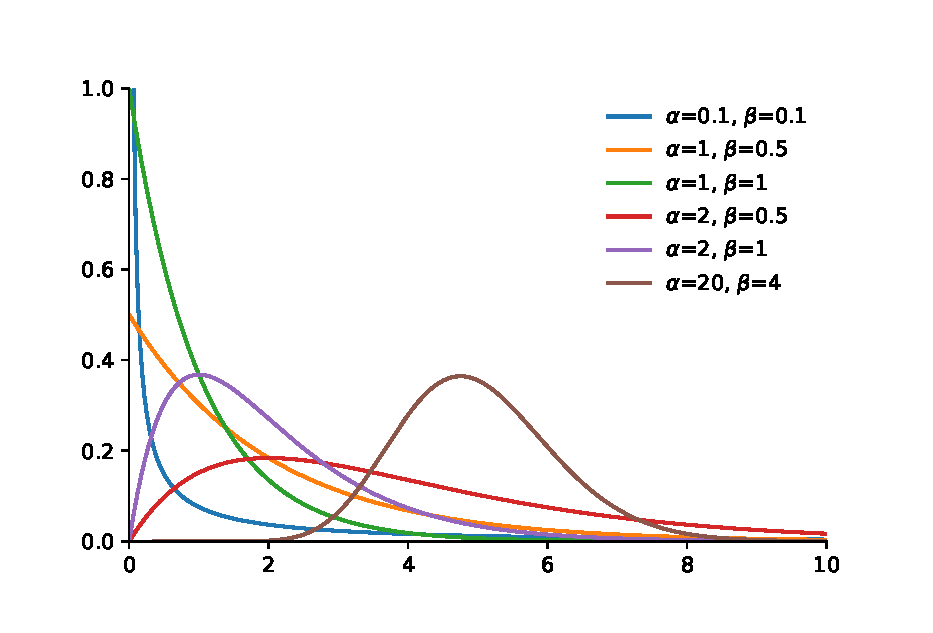
\includegraphics[width=0.8\textwidth]{ch2/gamma.eps}
    \caption{Función de densidad de probabilidad (pdf) de una distribución Gamma para diferentes parámetros de forma $\alpha$ y tasa $\beta$.}
    \label{img:gamma}
\end{figure}

En \citep{teh2005sharing} los parámetros de concentración se integran afuera usando un prior \textit{vague gamma} \citep{escobar1995bayesian}. Un prior \textit{vague gamma} es una distribución Gamma con una gran parte de la masa en torno a cero y una cola pesada (ver Figura \ref{img:gamma} para una ilustración de la pdf para diferentes parámetros). Por consecuencia, el prior tendrá un menor efecto de regularización y a medida que más datos se obtienen la posterior conincidirá con las observaciones empíricas. En este caso se utilizó un prior $\Gamma(\alpha=1, \beta=1)$.

\subsection{Interpretación de tópicos}

Los modelos de tópicos probabilísticos se caracterizan por tener un alto poder interpretativo, esto se debe a que la distribución de probabilidad de cada tópico sobre el vocabulario nos da una idea del tema al que pertenece, por otro lado, la mezcla de tópicos de cada documento nos muestra que tan importante es cada tópico en la generación de estos, como también dentro del corpus. \\

En este sentido, las visualizaciones nos pueden ayudar a interpretar mejor los resultados de los modelos de tópicos. Para la interpretación de los tópicos la metodología propuesta se basa en la herramienta de visualización desarrollada en  \citep{sievert2014ldavis}, la cual responde las siguientes preguntas, ¿Cuál es el significado de cada tópico?¿Cuán predominante es cada tópico?¿Cómo se relacionan los tópicos entre sí?\\

Para responder la pregunta 1 se incorpora un gráfico de barras que muestra las palabras más relevantes del tópico seleccionado dado un parámetro $\lambda \in [0,1]$. A través de una visualización espacial responde la pregunta 2 y 3. La visualización espacial consiste en aplicar técnicas de reducción de dimensionalidad como TSNE \citep{maaten2008visualizing} o PCA \citep{wold1987principal} (en este caso se utilizó TSNE) a la matriz de distancia entre tópicos, usando Jensen-Shannon divergence \citep{endres2003new} como médida de distancia. Una vez cada tópico es mapeado a un punto en un espacio de dos dimensiones se dibuja un círculo con centro en este punto y con radio proporcional a la cantidad de tokens generados por el tópico.\\
% se podría meter mano para reemplazar por WMD, en ese caso mover a una sección posterior

Para interpretar un tópico, lo usual es examinar una lista ordenada de las palabras más probables del tópico, usando ya sea desde cinco a treinta términos. Un problema frecuente que se presenta en este caso es que los términos que son comunes al corpus frecuentemente aparecen en el top de las palabras más probables de un tópico, haciendo difícil discernir el significado de estos. Para esto en \citep{sievert2014ldavis} se define una métrica denominada \textit{relevance}, la cual define la relevancia de una palabra no solo por su probabilidad dentro del tópico sino también por su exclusivad dentro del corpus. La \textit{relevance} de una palabra $w$ en el tópico $k$ dado $\lambda$ está dada a través de la siguiente expresión:

\begin{align}
    r(w,k|\lambda) = \lambda log (\phi_{kw})+ (1-\lambda)\lambda log\bigg(\frac{\phi_{kw}}{p_{w}}\bigg)
\end{align}

, donde $\lambda$ determina el peso que se le da a la probabilidad de la palabra $w$ dentro del tópico $k$ ($\phi_{kw}$) relativo a su \textit{lift}, el cual se define por el ratio entre la probabilidad de la palabra dentro del tópico y su probabilidad marginal a lo largo del corpus ($p_w$). Fijando $\lambda=1$ se obtiene el ranking de términos decrecientes en orden de su probabilidad dentro del tópico, y fijando $\lambda=0$ el ranking se basa solo en el \textit{lift}.

\section{Construcción del grafo temporal}
\label{ref:build_graph}

Nuestro objetivo no es solo descubrir tópicos sino también modelar sus interacciones en el tiempo, como nacimiento, muerte, evolución, divisón y fusión.
Así, la metodología propuesta se basa en la metodología descrita en la sección \ref{sec:similarity_graph} propuesta en \citep{beykikhoshk2018discovering}, debido que esta captura los dinamismos mencionados.\\

En general las medidas de similitud o distancia comparan vectores con el mismo dominio y dimensión, esto significa que los tópicos de épocas adyacentes deben compartir el mismo vocabulario. Matemáticamente, sea $\phi_{t, i}$ un tópico de la época $t$ y $V_{t}$ su vocabulario, sea  $\phi_{t+1, j}$ un tópico de la época $t+1$ y $V_{t+1}$ su vocabulario. Con una alta probabilidad existan palabras en $V_{t}$ que no están en $V_{t+1}$ y viceversa. Para poder comparar tópicos en épocas adyacentes se debe construir un vocabulario global $V_{t+1}^{'}=V_{t}\cup V_{t+1}$, luego aplicar $padding$ a los vectores $\phi_{t, i}$ y $\phi_{t+1, j}$, es decir, rellenar con ceros las posiciones que no están en el vocabulario de su dominio.\\

Una gran desventaja del enfoque anterior es que no captura similitud entre palabras, puesto que cada palabra ocupa una posición dentro del vector y no hay forma de comparar palabras que no son comúnes en ambas épocas. El peor caso sería considerar los vocabularios $V_{t}$ y $V_{t+1}$, con $V_{t}\cap V_{t+1} =  \emptyset$, a pesar de que cada palabra en $V_{t}$ tiene un sinónimo en $V_{t+1}$ la similitud entre tópicos entre las épocas $t$ y $t+1$ sería cero.\\

\subsection{Word Mover's Distance}

Para lidiar con el problema anterior, se propone utilizar una medida de distancia conocida como Word Mover's Distance (WMD) \citep{kusner2015word}, medida utilizada para comparar dos documento bajo una representación \textit{bag of words} a través de sus \textit{word embeddings} \citep{mikolov2013distributed}.\\

WMD calcula el costo mínimo de transformar un documento en otro, en esto caso particular sería el costo mínimo de llevar un tópico a otro. Para esto se resuelve el problema de transporte, donde los flujos son los pesos $\phi_{t,i}$ y $\phi_{t+1,j}$ y la matriz de costos es una matriz de distancia euclidiana entre los \textit{word embedding} de todas las palabras deS $V_{t}$ con $V_{t+1}$. En la Figura \ref{img:wmd_obama} se ilustra el espacio en el que viven las palabras de dos documentos.

\begin{figure}
    \centering
    \includegraphics[width=1\textwidth]{ch2/wmd-obama.png}
    \caption{Espacio vectorial de los \textit{word embeddings} de las palabras de dos documentos con un vocabulario de tamaño 4. Fuente: Figura de \citep{WMDPy}.}
    \label{img:wmd_obama}
\end{figure}

Sea  $V_{i}$ y $V_{j}$ los vocabularios del tópico $i$ y $j$ respectivamente, luego su WMD viene dado por $WMD(\phi_{i}, \phi_{j})$:

\begin{align}
\underset{x}{\text{min}}&\sum_{u \in V_{i}}\sum_{v \in V_{j}} c_{u,v}x_{u,v} \\ 
\textrm{s.t.} &\sum_{v \in V_{j}}x_{u,v}= \phi_{i,u}, \; u \in V_{i}\\ 
& \sum_{u \in V_{i}}x_{u,v}= \phi_{j,v}, \; v\in V_{j}\\
& x_{u,v} \geq 0,\; u \in V_{i} \;, v \in V_{j}\\ \nonumber
\end{align}

Donde $x_{u,v}$ es el flujo que va de la palabra $u$ del tópico $i$ a la palabra $v$ del tópico $j$, $\phi_{i,u}$ es la probabilidad de la palabra $u$ en el tópico $i$, $c_{u,v}$ es el costo de mover una unidad de flujo por el arco $(u,v)$, el costo entre palabras se mide como la distancia euclidiana entre los \textit{word embedding} de dichas palabras.\\

La primera restricción indica que el flujo que se mueve de una palabra $u$ del tópico $i$ a todas las palabras del tópico $j$ debe sumar su peso ($\phi_{i,u}$), la segunda restricción significa que el flujo que se mueve de una palabra $v$ del tópico $j$ a todas las palabras del tópico $i$ debe sumar su peso ($\phi_{j,v}$). Lo anterior implica que esta medida de distancia es simétrica, es decir, $WMD(\phi_{i}, \phi_{j}) = WMD(\phi_{j}, \phi_{i})$.\\

WMD se puede fácilmente transformar en una médida de similitud, $\rho(\phi_{i}, \phi_{j}) = \frac{1}{1+WMD(\phi_{i}, \phi_{j})}$, notar que si la WMD es 0 la similitud es 1 y si es $\infty$ la similitud es 0. \\

\subsection{WMD complejidad}

WMD es una medida de distancia intensiva en recursos computacionales. Para entender mejor esto utilizaremos la representación poliedral del problema, sea $N$ el tamaño del vocabulario entre dos épocas adyacentes, luego la región factible del problema anterior se puede representar como $\{x| Ax=b, x\geq 0\}$ sobre un grafo bipartito, con $A\in \mathbb{R}^{2N\times N^{2}}$ la matriz de incidencia, $b\in \mathbb{R}^{2N}$ la capacidad de los nodos y $x\in \mathbb{R}^{N}$ el flujo a enviar por cada uno de los arcos. Para resolver este problema se utilizó \citep{PyEMD}, la cual está basada en el algoritmo \citep{pele2009fast}, cuya complejidad del mejor tiempo promedio escala $\mathcal{O}(N^{2}log N)$.\\

Los tópicos siguen una distribución con forma de ley de potencia sobre el vocabulario, donde una pequeña fracción de las palabras concentran la mayor parte de la masa de la distribución. Además, en la práctica la interpretación de los tópicos se basa en los top $N$ palabras más probables con $N \in [5, 30]$, entonces, podemos aprovechar esta estructura para efectos de computar la WMD de un forma más eficiente, por ejemplo, utilizando solo las palabras que capturan un X\% de la distribución acumulada del tópico. De hecho si se reduce el vocabulario a un décimo esto traera en el peor caso promedio un \textit{speed up} de 200.\\

\subsection{Word Embeddings}

Computar WMD requiere contar con \textit{word embeddings}. Para estó se utilizó una de las más grandes colecciones de \textit{word embeddings} en español \citep{fastextSUC}, que cuenta con 1.313.423 \textit{embeddings}, colección obtenida utilizando el algoritmo FasText \citep{bojanowski2017enriching} sobre el corpus Spanish Unannotated Corpora (SUC) \citep{josecanneteSUC}, uno de los más grandes corpus de texto en español. FasText en comparación a otros enfoques para extraer \textit{embeddings} representa los \textit{tokens} a través de n-gramas de caracteres, de esta manera se pueden obtener \textit{embeddings} de \textit{tokens} no vistos durante el entrenamiento a partir de los \textit{embeddings} de los caracteres que lo componen.

\subsection{Métricas}

En la metodología propuesta podemos considerar dos fuentes de evaluación de desempeño, el descubrimiento de tópicos y cómo se relacionan. En ambos casos no se cuenta con el \textit{ground truth} para medir correctamente el desempeño. Si conocieramos el \textit{ground truth}, podríamos utilizar \textit{purity} \citep{manning2008introduction} para comparar la asignación de los documentos en torno a los tópicos con la etiqueta. En el caso del grafo temporal, si conocieramos las conexiones presentes y ausentes podríamos utilizar métricas de clasificación.\\

En \citep{blei2003latent,griffiths2004finding,cao2009density,arun2010finding,deveaud2014accurate,zhang2017lda} se describen algunas métricas que no requieren de una etiqueta, que pueden ser útil para realizar selección de modelo de tópico. Cabe destacar que estas métricas carecen de significado y sirven para comparar si un modelo de tópicos es superior a otro.\\

El trabajo propuesto no tiene por objetivo calibrar los hiperparámetros del HDP y se utilizó la configuración especificada en la sección \ref{sec:hdp_hiperparameters}. Por el contrario, se enfoca en medir el desempeño de las interacciones entre los tópicos descubiertos, asumiendo que los tópicos descubiertos están correctos. El desempeño es medido mediante métricas de clasificación sobre un grafo etiquetado. Esto es posible  debido a que el fenómeno de robo de vehículos no presenta muchos tópicos a diferencia de los tópicos latentes que podríamos encontrar en Wikipedia.\\

La métrica escogida en este caso es el \textit{macro average recall} \citep{forman2003extensive}, esta corresponde al promedio simple entre la tasa de aciertos de la clase presencia y ausencia de conexión. En general, debería haber más ausencia que presencia de conexión, así bajo esta métrica la clase presencia de conexión no será menospreciada, ya que el macro recall considera que el tasa de acertividad de ambas clases son igual de importantes.\\

Adicionalmente, al contar con un grafo etiquetado podemos observar el efecto de los hiperparámetros $\zeta$ y $q$ en la métrica de desempeño escogida. El hiperparámetro $\zeta\in[0,1]$ define el úmbral de corte, representa el punto operante de la cdf del grafo \textit{fully connected}, permite definir el cuantil que se usará como úmbral para eliminar arcos con similitud menor a este. El parámetro $q \in [0,1]$ define el soporte de los tópicos, utilizando aquellas palabras más probables que explican 100q\% de la distribución acumulada del tópico. 

\section{Resumen metodología}


\todo[inline]{Resumen metodología/Cuadro esquemático}

\chapter{Caso de estudio}
\label{ch:case_study}
\todo[inline]{Motivación}
\todo[inline]{Describir organización del contenido}

\todosec[inline]{Diseño del experimento}


\section{Datos}\todosec{Descripción del dataset: mejorar estilo y añadir ejemplos}

% Para este experimento se cuenta con las fuentes de datos de la Asociación de Aseguradores de Chile (AACH), corresponde a los relatos que las víctimas del robo de sus vehículos dan a las aseguradoras, lo cual corresponde a 49.015 relatos entre el 2011 y 2016.\\

% descripción detallada del conjunto de datos
% gráficos del Informe_1_fondef?
% hablar del nivel de granularidad, justificar en base facilidad de análisis de resultados, interpretación, largo del grafo, combinatoria, etc

% Para el uso de WMD es necesario contar con \textit{word embeddings}, para esto se utilizaron los \textit{embeddings} de \citep{fastextSBWC}, estos \textit{embeddings} fueron obtenidos utilizando el algoritmo FastText \citep{bojanowski2017enriching} sobre el corpus Spanish Billion Word Corpus (SBWC) \citep{cardellinoSBWCE}. FasText en comparación a otros enfoques para extraer \textit{embeddings} representa los \textit{tokens} a través de n-gramas de caracteres, de esta manera se pueden obtener \textit{embeddings} de \textit{tokens} no vistos durante el entrenamiento a partir de los \textit{embeddings} de los caracteres que lo componen.

\section{Procesamiento}

En esta sección se detallan los resultados de aplicar el procesamiento descrito en la sección \ref{sec:processing}. Con fines gráficos los resultados del procesamiento se decriben en un orden distinto al descrito en dicha sección, con el objetivo de mostrar en como estas afectan el tamaño del vocabulario. El orden es el siguiente, (i) tokenización (\textbf{t}), (ii) procesamiento de caracteres (\textbf{c}), (iii) eliminación de palabras poco frecuentes (\textbf{f}), (iv) filtro por vocabulario (\textbf{v}) y (v) eliminación de \textit{stopwords} (\textbf{s}).\\

En la Figura \ref{img:cum_dist1} se muestran la distribución acumulada del corpus original tras solo aplicar tokenización. En este caso los \textit{tokens} totales corresponden a 2.030.980 asociado a un vocabulario de 93.203 palabras.\\

La Figura \ref{im:cum_dist2} muestra los resultados al aplicar la etapa de procesamiento de caracteres, de esta se observa que se reduce el tamaño del vocabulario en cerca de la mitad, específicamente a 42.921 palabras, similarmente con la cantidad de tokens, que ahora son 1.028.412.

\begin{figure}
    \centering
    \includegraphics[width=0.8\textwidth]{ch3/cum_dist_1.eps}
    \caption{Frecuencia acumulada del vocabulario en orden decreciente de ocurrencia aplicando hasta el primer nivel de procesamiento.}
    \label{img:cum_dist1}
\end{figure}

\begin{figure}
    \centering
    \includegraphics[width=0.8\textwidth]{ch3/cum_dist_2.eps}
    \caption{Frecuencia acumulada del vocabulario en orden decreciente de ocurrencia aplicando hasta el segundo nivel de procesamiento.}
    \label{img:cum_dist2}
\end{figure}

Hasta este nivel de procesamiento se tiene que al menos el 50\% de las palabras ocurren una única vez y al menos un 80\% tiene una frecuencia igual o menor a 4. El 95\% de la distribución acumulada puede ser explicada con 7.837 palabras (un 18\% del vocabulario actual). En conclusión, la distribución de las palabras tiene una cola bastante pesada.\\

En la Figura \ref{img:cum_dist3} se muestra la nueva distribución tras eliminar las palabras que aparecen en menos del 0.1\% de los documentos de su época. En este nivel de procesamiento se redujo bastante el tamaño del vocabulario a 3.148 (al rededor de 14 veces) sin alterar tan significativamente la cantidad de tokens (alrededor de un 10\%), siendo ahora 925.693 tokens.\\

Luego se filtran palabras usando el vocabulario extraído del SUC. En la Figura Figura \ref{img_cum_dist4} se observa que el vocabulario se redujo a 2.902 y el corpus a 901.745 tokens. En este caso la variación no fue tan significativa, alrededor de un 8\% en el tamaño del vocabulario y de un 3\% en el caso del corpus.\\

Finalmente, se eliminan las \textit{stopwords}, de la Figura \ref{img:cum_dist5} se puede observar que esto significó una reducción significativa de tanto el vocabulario como en el tamaño del corpus, respectivamente en 32\%(1960 palabras) y 45\%(495182 \textit{tokens}). La reducción abrupta en la cantidad de \textit{tokens} se debe principalmente a que las \textit{stopwords} son parte de las palabras más frecuentes dentro del corpus.

\begin{figure}
    \centering
    \includegraphics[width=0.8\textwidth]{ch3/cum_dist_3.eps}
    \caption{Frecuencia acumulada del vocabulario en orden decreciente de ocurrencia aplicando hasta el tercer nivel de procesamiento.}
    \label{img:cum_dist3}
\end{figure}

\begin{figure}
    \centering
    \includegraphics[width=0.8\textwidth]{ch3/cum_dist_4.eps}
    \caption{Frecuencia acumulada del vocabulario en orden decreciente de ocurrencia aplicando hasta el cuarto nivel de procesamiento.}
    \label{img:cum_dist4}
\end{figure}

\begin{figure}
    \centering
    \includegraphics[width=0.8\textwidth]{ch3/cum_dist_5.eps}
    \caption{Frecuencia acumulada del vocabulario en orden decreciente de ocurrencia aplicando hasta el quinto nivel de procesamiento.}
    \label{img:cum_dist5}
\end{figure}

% El paso cero en el procesamiento de textos es tokenizar, la tokenización es una operación sobre una cadena de carácteres (\textit{string}) que consiste en dividir el \textit{string} en un conjunto de términos, en este caso la división se hizo por el carácter espacio, como resultado de esto se obtiene una lista de elementos, a cada elemento de esta lista se le denomina \textit{token} que en términos simples puede considerarse como una palabra para el ejemplo mencionado\todo{Mover a marco teórico}. \\

% Luego, en el primer nivel de procesamiento no interesa hacer distinción entre mayúsculas o minúsculas\footnote{En análisis de sentimiento puede ser interesante ya que las personas suelen expresar mensajes de enfado con letras capitales, por lo que las letras capitales añaden información al análisis.}, por ende, los carácteres de cada token son llevados a minúscula, también se eliminaron carácteres y tokens que no aportan información, como símbolos de puntuación, correos electrónicos y tokens que contienen números. En la figura \ref{img:cum_dist1} se observa la distribución acumulada de los tokens del corpus a este nivel de procesamiento, adicionalmente se tiene que el 50\% de los \textit{tokens} del vocabulario ocurren una sola vez, el 80\% tiene una ocurrencia menor o igual a 5 y el 95\% de la distribución acumulada puede ser explicada con 4199 \textit{tokens} (9\%) del vocabulario, se concluye que la distribución es sumamente pesada y es necesario recurrir a métodos adicionales para su reducción. \todo{Mover a marco teórico}\\











% En el segundo nivel de procesamiento se eliminaron las \texit{stopwords}, palabras que aportan poca información, como artículos, preposiciones y conectores, para esto se utilizó la lista de \textit{stopwords} disponible en el paquete NLTK de Python \citep{bird2009natural} la cual cuenta con 313 palabras. Además, esta lista de \textit{stopwords} se alimentó con \textit{stopwords} contextuales, palabras específicas del corpus que aportan poca información, para esto se hizó un etiquetado de las 1000 palabras más frecuentes del corpus incorporando 417 nuevas palabras, algunos ejemplos son palabras que hacen referencia a vehículo y robo, puesto que todos los documentos corresponden a robos de vehículos.\todo{Mover a marco teórico}\\

% El tercer nivel de procesamiento consiste en normalizar los tokens para reducir aún más el vocabulario, como métodos de normalización los más utilizados son \textit{stemming}  y lematización. \textit{Stemming} es el proceso de llevar una palabra a su raíz (\textit{stem}), en la práctica \textit{stemming} consiste en aplicar un algoritmo basado en ciertas reglas gramáticales para extraer sufijos \citep{porter1980algorithm}, como desventaja es que stemming no tiene en cuenta el contexto de la palabra por lo que la raíz obtenida puede no corresponder a la raíz verdadera de la palabra, además, para el caso de modelamiento de tópicos los tópicos se vuelve más difícil de interpretar, ya que palabras con significado completamente distinto terminan con la misma raíz o bien la raíz encontrada no tiene un significado claro. Por otro lado, lematización es el proceso de agrupar juntas las formas flexionadas de una palabra para que puedan analizarse como un elemento, identificado como lema, su diferencia principal con \textit{stemming} es que opera con conocimiento del contexto de la palabra para discriminar entre palabras que tienen significado diferente dependiendo del \textit{part of speech tagging} (POST) y de una tabla de búsqueda (\textit{lookup table}). Como método de normalización se decidió utilizar lematización en vez de \texit{stemming} debido a que tiene menos impacto en la interpretación de los tópicos, sin embargo es una operación más intensiva debido a que \texit{stemming} es un algoritmo basado en reglas simples mientras que en lematización se suele usar redes neuronales recurrentes (RNNs) para el POST y una vez determinadas las etiquetas gramaticales de las palabras en un documento se utiliza una \textit{lookup table} para encontrar el lema correspondiente. La implementación de lematización utilizada es la implementación de lematización en español del paquete spaCy de Python \citep{spacy2}.\todo{Mover a marco teórico}\\

% El cuarto y último nivel de procesamiento corresponde a eliminar tokens con baja frecuencia, puesto que el modelo no será capaz de levantar patrones en tokens que aparecen una única vez o con una ocurrencia poco significativa, luego, como el corpus está particionado en épocas, se eliminaron aquellos tokens que aparecen en menos de 5 documentos dentro de una época.\todo{Mover a marco teórico}

% En la figura \ref{img:cum_dist2} se presenta la distribución acumulada del vocabulario hasta el cuarto nivel de procesamiento, en donde se observa que la cola de distribución es bastante menos pesada que bajo el primer nivel de procesamiento, además, como se observa en la tabla \ref{table:processing_stats} el tamaño del vocabulario se redujo a menos de un décimo del vocabulario obtenido bajo el primer nivel de procesamiento y es menos de un décimo del tamaño del corpus, por lo que bajo este nivel de procesamiento es posible desarrollar modelos con mayor fuerza estadística.\todoredo{Rehacer}

% \begin{table}[H]
%     \begin{tabular}{|c|r|r|r|}
%         \hline
%         procesamiento & \multicolumn{1}{c|}{documentos} & \multicolumn{1}{c|}{vocabulario} & \multicolumn{1}{c|}{tokens} \\ \hline
%         raw          & 49.015                           & 79.327                            & 2.030.980                     \\ \hline
%         ch    & 49.011                           & 46.708                            & 1.947.235                     \\ \hline
%         ch+s+l+f      & 47.993                           & 4.106                             & 508.987                      \\ \hline
%         \end{tabular}
%     \caption{Estadísticas del corpus bajo distintos niveles de procesamientos, \textbf{raw}: sin procesamiento, \textbf{ch}: eliminación de símbolos de puntuación, correos electrónicos y tokens con números, \textbf{ch+s+l+f}: además incluye eliminación de stopwords (s), lemmatización (l) y eliminación de tokens con baja ocurrencia (f).}
%     \label{table:processing_stats}
% \end{table}\todoredo{Rehacer}

% En la tabla \ref{table:innovation_rate} se muestra el detalle del vocabulario para cada una de las épocas tras procesar el corpus, de aquí se extrae que en promedio un 21.28\% del vocabulario se olvida de una época a otra y un 28.19\% es nuevo, es otras palabras, en promedio alrededor de un 50\% del vocabulario no es común entre tópicos de épocas adyacentes, esto justifica la necesidad de utilizar médidas de similitud que capturen la similitud entre palabras de épocas adyacentes ante la renovación que sufre el vocabulario en el tiempo.\todoredo{Rehacer}

% \begin{table}[h]
%     \begin{tabular}{|r|r|r|r|r|}
%     \hline
%     \textbf{época} & \textbf{old\_vocab} & \textbf{new\_vocab} & \textbf{\%old\_vocab} & \textbf{\%new\_vocab} \\ \hline
%     2              & 1.919                     & 1.986                     & 23,35                 & 26.84                 \\ \hline
%     3              & 1.986                     & 2.092                     & 22,61                 & 27.95                 \\ \hline 
%     4              & 2.092                     & 2.414                     & 18,21                 & 33.60                 \\ \hline
%     5              & 2.414                     & 2.629                     & 19,80                 & 28.71                 \\ \hline
%     6              & 2.629                     & 2.666                     & 22,44                 & 23.85                 \\ \hline
%     \end{tabular}
%     \caption{Evolución del vocabulario en el tiempo, \textbf{old\_vocab}: corresponde al vocabulario del período $t-1$, \textbf{new\_vocab}: corresponde al vocabulario del período $t$, \textbf{\%old\_vocab}: porcentaje de tokens del período $t-1$ que ya no están en el período $t$ y \textbf{\%new\_vocab}: porcentaje de tokens del período $t$ que no están en el período $t-1$.}
%     \label{table:innovation_rate}.
% \end{table}\todoredo{Rehacer}

\section{Análisis cuantitativo de resultados}
\todoredo[inline]{Rehacer}

% Al aplicar HDP de forma independiente en cada una de los épocas se obtuvo el siguiente número de tópicos [8, 10, 9, 8, 8, 9].

% \subsubsection{Distribución acumulada de los tópicos}
% En la figura \ref{img:cum_dist3} se muestra la distribución acumulada promedio de los tópicos, se tiene que en promedio un 8.54\% y 21.42\% del vocabulario se puede capturar un 80\% y 95\% respectivamente de la distribución acumulada de los tópicos, además, para un 99\% de los tópicos basta con un 37\% del vocabulario para capturar el 95\% de su distribución acumulada, por tanto, una representación incompleta de los tópicos usando las palabras más probables que capturan el 80\% de la distribución acumulada trae consigo una disminución importante en el tamaño del vocabulario\todoredo{Rehacer}. 

% \begin{figure}
%     \centering
%     \includegraphics[width=0.8\textwidth]{ch3/cum_dist_3.png}
%     \caption{Distribución acumulada promedio de los tópicos en función del vocabulario. El punto (x,y) en el gráfico corresponde a la fracción x del vocabulario que explica la fracción y de la distribución acumulada del tópico. Los puntos corresponden a los cuantiles 60\%, 80\%, 90\%, 95\% y 99\%.}
%     \label{img:cum_dist3}
% \end{figure}\todoredo{Rehacer}

% \subsubsection{Construcción del grafo temporal}

% El modelo propuesto considera tres hiperparámetros:
% \begin{itemize}
%     \item $q \in [0,1]$: para el cálculo de WMD se utilizan las palabras más probables del tópico que explican un 100q\% de la distribución acumulada del tópico. Este parámetro genera un nuevo tópico (se normaliza para sumar 1) con un vocabulario más reducido.
%     \item $\lambda \in [0,1]$: este parámetro pondera la probabilidad de la palabra dentro del tópico con su exclusividad. El nuevo tópico generado es normalizado para sumar 1.
%     \item $\zeta \in [0,1]$: punto operante de la cdf del grafo inicial, permite definir el cuantil que se usará como úmbral para eliminar arcos con similitud menor a este. 
% \end{itemize}\todo{Marco teórico}

% Para entender de mejor manera la influencia de cada uno de estos parámetros se hizó un etiquetado de los arcos del grafo temporal, asignando un 1 a los arcos que deberían estar presente y 0 a los que no. Luego, se hizó una búsqueda a través de la siguiente grilla de parámetros, $\lambda \in \{0.2, 0.4, 0.6, 0.8, 1.0\}$, $q \in \{0.2, 0.4, 0.6, 0.8, 0.9, 0.95\}$ y $\zeta \in \{0.05, 0.10, ..., 0.90, 0.95\}$. \todo{Marco teórico y diseño de experimento}\\

% Como métrica de evaluación se propone \textit{F-score}, definida por:
% \begin{align}
%     F-score = 2\times \frac{\text{precision}\cdot \text{recall}}{\text{precision}+\text{recall}}
% \end{align}
% \todoredo{Usar métrica acorde al marco teórico}
% , donde \textit{recall} es la tasas de acierto sobre la clase positiva (presencia de un arco) y \textit{precision} es la tasa de acierto de las predicciones sobre la clase positiva. Esta métrica permite balancear la acertividad con la precisión, así una configuración que no pode ningún arco tendra un \textit{recall}=1, pero un bajo \textit{precision} (notar que el númerador decrece más rápido que el denominador). \\

% De la figura \ref{img:f_score} se observa que \textit{F-score} tiende a ser creciente en función de $\zeta$, esto se debe a que menor $\zeta$ más falsos positivos (pues son más arcos los que sobreviven) empeorando así el \textit{precision} y por consecuencia el \textit{F-score}. Las configuraciones óptimas ocurren en su mayoría en $\zeta=0.95$ con excepción de tres configuraciones de las treinta posibles de $q\times \lambda$, las cuales se dan en $\zeta=0.9$ para los parámetros $q=0.2$ con $\lambda \in \{0.8, 1\}$ y $q=0.4$ con $\lambda=0.2$, sin embargo, el valor óptimo alcanzado es bastante cercano al obtenido con $\zeta=0.95$. En cuanto a $\lambda$ se observa que no existen muchas diferencias entre $\lambda\in\{0.6, 0.8, 1.0\}$ a diferencia de $\lambda \in \{0.2, 0.4\}$ que suele estar significativamente por debajo de las otras curvas, además se observa una dominancia débil en $\lambda$, es decir, en el $\zeta$ óptimo dado un $(q, \lambda)$ un $\lambda$ mayor no es peor. En el caso del parámetro $q$ se observa que para $q\geq 0.6$ el óptimo obtenido para $\lambda\geq 0.4$ es el mismo, en cambio para $q=0.4$ esto se cumple para todo $\lambda\geq 0.6$ y con $q=0.2$ para $\lambda \geq 0.8$.\todoredo{Rehacer} 

% \begin{figure}
%     \centering
%     \includegraphics[width=1\textwidth]{ch3/f_score.png}
%     \caption{F-score (eje vertical) para diferentes configuraciones de los hiperparámetros $q$, $\zeta$ (eje horizontal) y $\lambda$.}
%     \label{img:f_score}
% \end{figure}\todoredo{Rehacer}

% De la tabla \ref{table:f_score} se observa que la configuración óptima se alcanza con $q=0.2$ con $\zeta=0.9$, además esto ocurre tanto para $\lambda=0.8$ como $\lambda=1.0$, por lo que es escoje la configuración $(q, \zeta, \lambda) = (0.2, 0.9, 1.0)$ para construir el grafo temporal. En la figura \ref{img:cdf} se observa la distribución acumulada de la similitud para el grafo completamente conectado, por lo que el para $zeta=0.9$ el úmbral viene siendo 0.21.\todoredo{Rehacer}

% \begin{table}[H]
%     \begin{tabular}{|c|c|c|c|c|}
%     \hline
%     \textbf{q} & \textbf{zeta} & \textbf{recall} & \textbf{precision} & \textbf{f-score} \\ \hline
%     0.2        & 0.9           & 0.87            & 0.71               & 0.78             \\ \hline
%     0.4        & 0.95          & 0.61            & 1                  & 0.76             \\ \hline
%     0.6        & 0.95          & 0.61            & 1                  & 0.76             \\ \hline
%     0.8        & 0.95          & 0.61            & 1                  & 0.76             \\ \hline
%     0.9        & 0.95          & 0.61            & 1                  & 0.76             \\ \hline
%     0.95       & 0.95          & 0.61            & 1                  & 0.76             \\ \hline
%     \end{tabular}
%     \caption{Configuración de $\zeta$ para cada $q$ que máximiza el \textit{F-score}.}
%     \label{table:f_score}
% \end{table}\todoredo{Rehacer}

% \begin{figure}
%     \centering
%     \includegraphics[width=0.8\textwidth]{ch3/cdf.png}
%     \caption{Estimación empírica de la función de distribución acumulada (cdf) de la similitud entre tópicos correspondiente al grafo temporal completamente conectado para la configuración óptima $(q, \lambda)=(0.2, 1.0)$.}
%     \label{img:cdf}
% \end{figure}\todoredo{Rehacer}

% En la figura \ref{img:speedup} se observa que la configuración óptima es en promedio 184 veces más eficiente que $q=0.95$, esto se debe a que $q=0.2$ es un 0.3\% del vocabulario (6 palabras en promedio) y $q=0.95$ alrededor de un 21\% (488 palabras en promedio).\todoredo{Rehacer}


% \begin{figure}
%     \centering
%     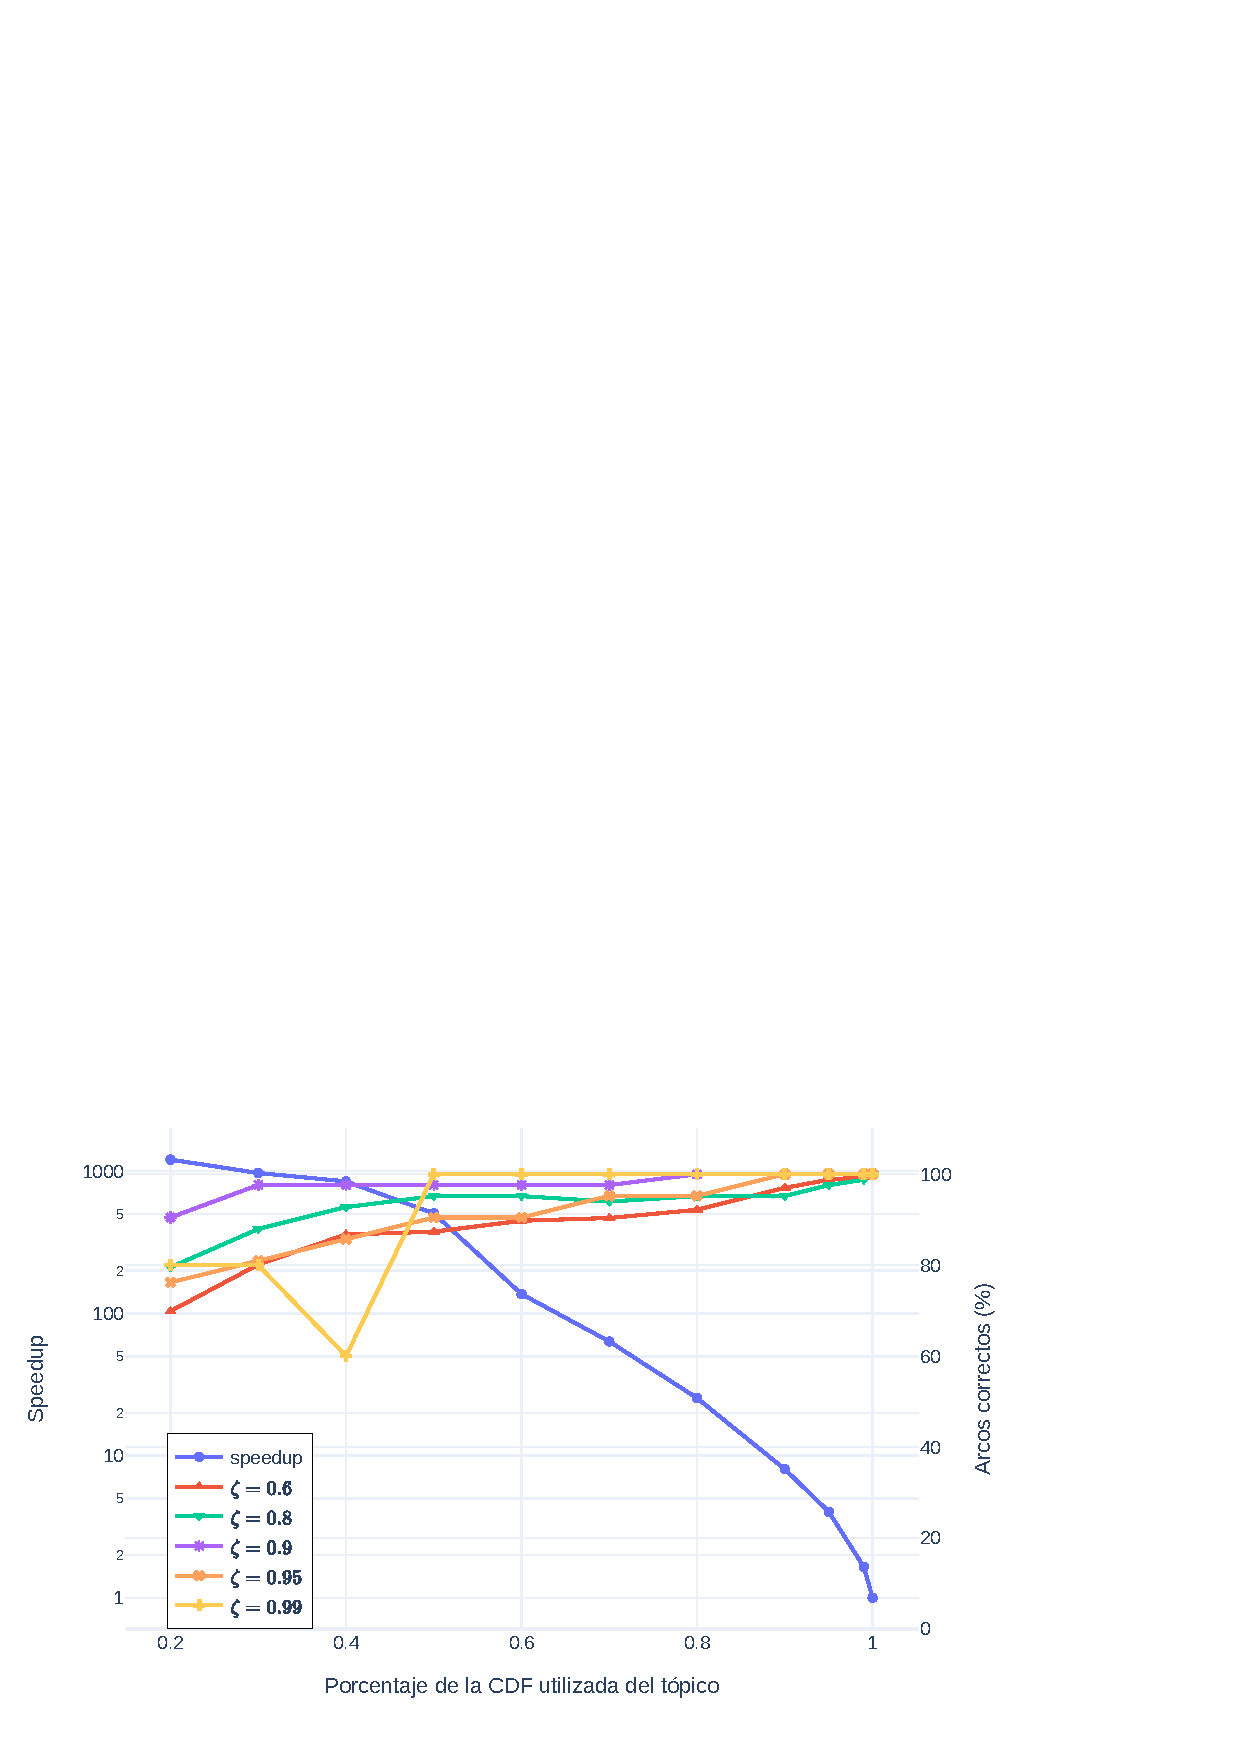
\includegraphics[width=1\textwidth]{ch3/speedup.png}
%     \caption{Speedup promedio de la construcción del grafo en función de $q$. El speedup 1 equivale al tiempo más lento el cual está asciado a $q=0.95$ que es el valor de $q$ más grande y por ende con menor reducción de vocabulario de los tópicos a la hora de computar WMD.}
%     \label{img:speedup}
% \end{figure}\todoredo{Rehacer}

% %\ref{img:ground_truth} y \ref{img:pruned_graph}
% %conteo de arcos y blabla
% %asociacion a tamaño de los topicos 
% %no hablar todavía del significado de los tópicos

% \begin{figure}
%     \centering
%     \includegraphics[width=0.8\textwidth]{ch3/ground_truth.png}
%     \caption{Grafo temporal etiquetado.}
%     \label{img:ground_truth}
% \end{figure}\todoredo{Rehacer}

% \begin{figure}
%     \centering
%     \includegraphics[width=0.8\textwidth]{ch3/pruned_graph.png}
%     \caption{Grafo temporal obtenido a partir de la configuración óptima de parámetros $(q, \lambda, \zeta) = (0.2, 1.0, 0.9)$.}
%     \label{img:pruned_graph}
% \end{figure}\todoredo{Rehacer}

\section{Análisis cualitativo de resultados}
\todosec[inline]{Análisis cualitativo de tópicos}

\chapter{Conclusiones y trabajo futuro}
\label{ch:conclusion}
\todosec[inline]{Conclusiones}

\todosec[inline]{Otras aplicaciones}

\todosec[inline]{Trabajo futuro}

\bibliography{main}

% FIN DEL DOCUMENTO
\end{document}
